\documentclass{cumcmthesis}

\usepackage[framemethod=TikZ]{mdframed}
\usepackage{url}   % 网页链接
\usepackage{subcaption} % 子标题

% 公式编号按节自动编号：(5.1)(5.2)……；图表编号同样跟随节（图5.1、表5.1）
\numberwithin{equation}{section}
\numberwithin{figure}{section}
\numberwithin{table}{section}
% cls 中 \thesection 为中文（五、），此处强制公式/图表前缀使用阿拉伯数字
\renewcommand{\theequation}{\arabic{section}.\arabic{equation}}
\renewcommand{\thefigure}{\arabic{section}.\arabic{figure}}
\renewcommand{\thetable}{\arabic{section}.\arabic{table}}

% 第一问、第二问增强图表所在目录
\graphicspath{{../求解代码/第一问/figures_enhanced/}{../求解代码/第二问/figures_enhanced/}}
\title{基于模型的问题研究}
\tihao{A}
\baominghao{xxxx}
\schoolname{XX大学}
\membera{ }
\memberb{ }
\memberc{ }
\supervisor{ }
\yearinput{2025}
\monthinput{09}
\dayinput{04}

\begin{document}

% \maketitle
\makeatletter 
\begin{center}
    {\huge \bfseries \@title}
\end{center}

 \begin{abstract}
    本文针对穿越沙漠的小游戏进行研究。

\keywords{\TeX{}\quad  图片\quad   表格\quad  公式}
\end{abstract}

\section{问题重述}

本题对一个沙漠游戏的最优决策问题展开讨论。玩家从起点出发在有限时间内到达终点并以剩余资金最大化为目标取得胜利。
游戏过程中，玩家需要在天气、负重、水和食物影响下合理规划路线、停留地点、资源购买以及矿山挖矿等行为。

基本规则如下：

（1）时间以天为单位，第0天玩家位于起点。玩家必须在截止日期或之前到达终点，到达终点后游戏结束。

（2）穿越沙漠需要水和食物两种资源，最小计量单位均为箱。每天玩家携带的水和食物总质量不能超过负重上限。如果在到达终点前水或食物耗尽，则视为游戏失败。

（3）每天天气为“晴朗”“高温”“沙暴”三种状况之一，沙漠中所有区域的天气相同。

（4）每天玩家可以从所在区域移动到相邻区域，也可以原地停留；沙暴日必须原地停留。

（5）玩家原地停留一天消耗的资源量称为基础消耗量；行走一天消耗的资源量是基础消耗量的相应倍数。

（6）第0天玩家可在起点用初始资金按基准价格购买水和食物。玩家可以停留在起点或返回起点，但不能多次在起点购买资源。到达终点后，剩余的水和食物可以退回，每箱退回价格为基准价格的一半。

（7）玩家在矿山停留时，可以通过挖矿获得资金，挖矿一天获得的资金称为基础收益。若挖矿，当天消耗的资源量是基础消耗量的相应倍数；若不挖矿，则消耗基础消耗量。到达矿山当天不能挖矿。沙暴日也可以挖矿。

（8）玩家经过村庄或在村庄停留时，可以用剩余的初始资金或挖矿所得资金随时购买水和食物，每箱价格为基准价格的2倍。

请根据游戏的不同设定建立数学模型，解决以下问题：

问题一：假设只有一名玩家，且整个游戏时段内每天天气状况事先全部已知，试给出一般情况下玩家的最优策略。求解附件中的“第一关”和“第二关”，并将相应结果分别填入Result.xlsx。

问题二：假设只有一名玩家，玩家仅知道当天天气状况，并可据此决定当天行动方案，试给出一般情况下玩家的最佳策略，并对附件中的“第三关”和“第四关”进行具体讨论。

问题三：现有$n$名玩家，初始资金相同，且同时从起点出发。若某天其中任意$k(2\leq k \leq n)$名玩家均从区域A行走到相邻区域B（B$\neq$A），则他们中任一人的资源消耗量均为基础消耗量的3倍；若某天其中任意若干名玩家在同一矿山挖矿，则他们中任一人的资源消耗量均为基础消耗量的$2k$倍，且每名玩家当天通过挖矿获得的资金为基础收益的$\frac{1}{k}$；若某天其中任意$k(2\leq k \leq n)$名玩家在同一村庄购买资源，则每箱价格均为基准价格的4倍。其他情况下资源消耗量和资源价格与单人游戏相同。

（1）假设整个游戏时段内每天天气状况事先全部已知，每名玩家的行动方案需在第0天确定且此后不能更改。试给出一般情况下玩家应采取的策略，并对附件中的“第五关”进行具体讨论。

（2）假设所有玩家仅知道当天天气状况，从第1天起，每名玩家在当天行动结束后均知道其余玩家当天的行动方案和剩余资源数量，并确定各自第二天的行动方案。试给出一般情况下玩家应采取的策略，并对附件中的“第六关”进行具体讨论。

注1：附件地图中，有公共边界的两个区域称为相邻；仅有公共顶点而没有公共边界的两个区域不视为相邻。

注2：Result.xlsx中剩余资金数（剩余水量、剩余食物量）指当日所需资源全部消耗完毕后的资金数（水量、食物量）。若当日还有购买行为，则指完成购买后的资金数（水量、食物量）。

\section{问题分析}
        \subsection{问题一的分析}
        问题一需要求解在天气已知、时间有限、位置离散、资源受限且途中可进行补给与矿山产生收益的情况下进行决策。
        因此，不能简单追求最短路径或最高收益，必须进行联合优化。首先将最短路径设置为下界，由于同一时间、同一位置可以由不同历史路径到达，而后续最优决策仅取决于当前所剩资源与现金，满足Bellman最优子结构。
        据此以天为阶段，以位置、水量、食物量为状态，以现金为价值函数，逐日枚举停留、行走与挖矿的情况：若当天在村庄结束则补充购买，若达到终点则将剩余资源折合成现金。同时为控制计算量，通过Pareto支配、最早到达日与乐观收益作为上界剔除不可能最优状态。
        最终得到逐日最优策略。
        \subsection{问题二的分析}
        问题二在问题一的基础上改变天气条件，将天气状况改为未知后进行决策。本文通过构造满足“仅知当天”的非前视反馈策略并进行反馈优化完成求解。
        首先，第三关与第四关给出了对应的不确定性结构：第三关明确10日内无沙暴且未来仅有晴朗与高温两种天气，可穷举构造1024种情景；第四关仅知“30日内沙暴较少”，故将沙暴天数作为可扫描的预算参数构造不确定集。
        据此以天为阶段，以位置、水量、食物量、现金与天气情况为状态，以最终财富（现金与剩余资源半价回收）为价值函数，逐日枚举移动、停留、挖矿与补给动作，
        用在未来所有天气分支中最不利分支的后续最优值形成自适应鲁棒Bellman递推，得到动态规划路线。同时借助Pareto、时间下界与资源上界剪枝剔除不可能最优状态，并以题内30日天气样本估计的经验Markov模型作名义期望并列判别，以完全信息Oracle与蒙特卡洛交叉验证策略的稳健性与近优性，最终得到最优策略。
        \subsection{问题三的分析}
\section{模型假设}
\section{符号说明}

\section{模型建立与求解}
\subsection{问题一的模型建立与求解}
    \subsubsection{动态规划模型}

    对于问题一，最短路径只能描述简单的空间距离，无法考虑天气、资源、现金收益的影响。但动态规划具备最优子结构：即只需保存每个状态下的最大现金而无需记录完整路径历史便可以进行精确求解。
    
    \begin{enumerate}
        \item\textbf{图模型}
        
        
        \hspace*{2em}首先将沙漠地图表示为无向图 $G=(V,E)$。若区域 $i$ 与 $j$ 存在公共边界，则 $(i,j)\in E$；仅有公共顶点不连边。每次移动恰好占用一个可移动日，因此边权统一为 1。定义邻接集合 $N(i)=\{j\mid (i,j)\in E\}$。BFS 仅用于计算各节点到终点的最少移动步数 $d(i,g)$，作为可达性下界；具体哪天移动、是否停留或挖矿，由动态规划决定。第一关共 27 个节点、53 条无向边；第二关共 64 个节点、161 条无向边。

        \item\textbf{状态变量与价值函数}
        
        \hspace*{2em}以天为阶段，将玩家处境抽象为“日期---位置---水量---食物量”四元状态，现金不作为状态维度，而由价值函数保存：

\begin{equation}
S_t = (t,\ i_t,\ W_t,\ F_t)
\label{eq:q1_state}
\end{equation}

\hspace*{2em}其中，$t$ 为当前日序号，$i_t$ 为日末所在区域，$W_t$ 和 $F_t$ 分别为日末剩余水和食物的箱数。

\begin{equation}
V_t(i,\ w,\ f) = \text{第 }t\text{ 日日末处于节点 }i\text{、余水 }w\text{、余食 }f\text{ 时可达到的最大现金}
\label{eq:q1_value}
\end{equation}

\hspace*{2em}
其中，$V_t$ 即该状态的价值函数。

        \item\textbf{目标函数}
        
        \hspace*{2em}
        题目允许到达终点后按基准价的一半退回剩余水和食物，因此不能预先假设终点库存为零。对任意不晚于截止日期 $T$ 的终点状态，终端总财富为到达时的现金加上剩余资源的半价回收价值：

\begin{equation}
\max Z = C_\tau + 0.5\,p_w\,W_\tau + 0.5\,p_f\,F_\tau
\label{eq:q1_obj}
\end{equation}
\begin{equation}
\text{s.t.}\quad 0 \leq \tau \leq T,\quad i_\tau = g
\label{eq:q1_objcon}
\end{equation}

\hspace*{2em}
其中，$Z$ 为终端总财富；$C_\tau$ 为到达终点当天的现金；$W_\tau$ 和 $F_\tau$ 为终点库存；$p_w$ 和 $p_f$ 分别为水和食物的基准价格。采用价值函数后，最终目标写为：

\begin{equation}
Z^* = \max_{0 \leq t \leq T,\ w,\ f} \Bigl\{ V_t(g,\ w,\ f) + 0.5\,p_w\,w + 0.5\,p_f\,f \Bigr\}
\end{equation}

        \item\textbf{约束条件} 
        

        \begin{enumerate}
            \item\textbf{ 初始采购}
            
             \hspace*{2em}第 0 天仅在起点按基准价采购一次：

\begin{equation}
V_0(s,\ w,\ f) = C_0 - p_w\,w - p_f\,f
\label{eq:q1_init}
\end{equation}
\begin{equation}
p_w\,w + p_f\,f \leq C_0,\quad m_w\,w + m_f\,f \leq M,\quad w,\ f \in \mathbb{Z}_+
\label{eq:q1_initcon}
\end{equation}

其中，$C_0$ 为初始资金，$m_w$ 和 $m_f$ 分别为每箱水和食物的质量，$M$ 为负重上限。玩家后续即使返回起点，也不再生成起点购买转移。

            \item \textbf{行动与消耗} 
            
            \hspace*{2em}停留、行走、挖矿的消耗倍率分别为 1、2、3。沙暴日禁止移动，但停留和矿山挖矿仍允许；到达矿山当天不能挖矿——由于动态规划从"前一日结束状态"向下一日扩展，挖矿动作只从"前一天已在矿山"的状态生成，因此该规则满足：

\begin{equation}
\kappa(a_t) = \begin{cases}
1, & a_t = \text{停留} \\
2, & a_t = \text{行走} \\
3, & a_t = \text{挖矿}
\end{cases}
\label{eq:q1_kappa}
\end{equation}
\begin{equation}
\Delta W_t = \kappa(a_t)\,c_w(\omega_t),\quad \Delta F_t = \kappa(a_t)\,c_f(\omega_t)
\label{eq:q1_consume}
\end{equation}
\begin{equation}
\text{行走可行} \Leftrightarrow (i,j)\in E\text{ 且 }\omega_t \neq \text{沙暴}
\label{eq:q1_move}
\end{equation}
\begin{equation}
\text{挖矿可行} \Leftrightarrow i \in V_m
\label{eq:q1_mine}
\end{equation}

\hspace*{2em}其中，$c_w(\omega_t)$ 和 $c_f(\omega_t)$ 分别为天气 $\omega_t$ 下水、食物的基础消耗，$V_m$ 为矿山节点集合。

            \item\textbf{资源与现金递推} 
            
            \hspace*{2em}扣除当日消耗后，若挖矿则增加基础收益 $R$，否则现金不变；若在村庄则执行补给：

\begin{equation}
W_t = W_{t-1} - \Delta W_t + b^w_t,\quad F_t = F_{t-1} - \Delta F_t + b^f_t
\label{eq:q1_res}
\end{equation}
\begin{equation}
C_t = C_{t-1} + R\cdot{I}(a_t = \text{挖矿}) - 2\,p_w\,b^w_t - 2\,p_f\,b^f_t
\label{eq:q1_cash}
\end{equation}
\begin{equation}
W_t \geq 0,\quad F_t \geq 0,\quad C_t \geq 0
\label{eq:q1_rescon}
\end{equation}
\begin{equation}
m_w\,W_t + m_f\,F_t \leq M
\label{eq:q1_load}
\end{equation}

其中，$b^w_t$ 和 $b^f_t$ 为日末村庄购买量，非村庄节点处为零；${I}(\cdot)$ 为指示函数。

        \end{enumerate}

        \item\textbf{Bellman 状态转移}
        
        \hspace*{2em}设从状态 $s=(t-1,i,w,f)$ 经动作 $a$ 和购买 $b$ 到达 $s'=(t,j,w',f')$，现金增量为 $r_t(s,a,b)$，则：

\begin{equation}
V_t(j,\ w',\ f') = \max\Bigl\{ V_t(j,\ w',\ f'),\ V_{t-1}(i,\ w,\ f) + r_t(s,\ a,\ b) \Bigr\}
\label{eq:q1_bellman}
\end{equation}

若目标节点为终点，则在更新 $V_t$ 后立即计算终端财富，不再将状态扩展到下一天。
    \end{enumerate}
\subsubsection{压缩状态空间支配剪枝}

完整动态规划在理论上需要枚举约 $T \times |V| \times W_{\max} \times F_{\max}$ 个状态，远超实际可达范围。为此采用三种剪枝策略，不改变全局最优解。

\textbf{（1）Pareto 状态支配剪枝}

在同一日 $t$、同一节点 $i$，若存在两个标签 $A=(w_A,f_A,C_A)$ 和 $B=(w_B,f_B,C_B)$，且 $A$ 的水、食物和现金均不低于 $B$，则称 $A$ 支配 $B$：

\begin{equation}
A \succcurlyeq B \ \Leftrightarrow\ w_A \geq w_B,\ f_A \geq f_B,\ C_A \geq C_B,\ \text{且至少一个严格大于}
\label{eq:dominate}
\end{equation}

从 $B$ 出发的任意后续合法策略都要求消耗非负数量的水和食物并支付非负的采购费用。$A$ 拥有不少于 $B$ 的库存和现金，可以选择与 $B$ 相同的行动；若 $B$ 未来需要采购，$A$ 可购买相同或更少的数量以达到不低于 $B$ 的库存，因此不会因负重约束而变得更差。到终点后额外库存还具有非负回收价值，故 $A$ 的最终财富不低于 $B$，删除 $B$ 不会删掉最优解。

实现时不为每个 $(t,i)$ 建立完整水-食物矩阵，而是用稀疏字典保存已出现的标签，在每一层更新结束后维护非支配前沿。

\textbf{（2）沙暴修正的最早到达日剪枝}

传统最短路下界只检查"剩余天数是否不少于最短步数"，但第一问未来沙暴日完全已知，沙暴日绝对不能移动，因此可构造更强的确定可达性下界。

令 $d = d(i,g)$ 为当前节点到终点的最短移动步数。从第 $t$ 天结束状态出发，需要在未来找到至少 $d$ 个非沙暴日完成 $d$ 次移动。定义 $e(t,d)$ 为满足下式的最小日期 $q$：

\begin{equation}
\sum_{k=t+1}^{q} I(\omega_k \neq \text{沙暴}) \geq d
\label{eq:sand_arrival}
\end{equation}

若直到截止日 $T$ 仍不存在这样的 $q$，则当前状态即使忽略资源限制也无法到达终点，可立即删除。该剪枝不依赖任何经验参数，完全由题目已知天气序列确定。

\textbf{（3）乐观收益上界剪枝}

当已经获得一个可行终点财富 $Z_{\text{best}}$ 后，对任意中间状态构造极度乐观的收益上界。假设玩家从现在起不再花钱补给、现有资源最后都能按半价回收，且剩余每一天都能获得一次基础挖矿收益 $R$：

\begin{equation}
\text{UB} = C + \frac{1}{2}\,p_w\,W + \frac{1}{2}\,p_f\,F + (T - t)\,R
\label{eq:ub}
\end{equation}

真实策略不可能比该上界更高，因为实际还需移动消耗资源，且不可能每天都在矿山挖矿。若 $\text{UB} \leq Z_{\text{best}}$，则当前状态无法改善最优解，安全剪枝。该上界全部来自题目给定参数，无人为权重。

\subsubsection{求解结果}

两关均由 SciPy \texttt{milp} 接口调用 HiGHS 求解器，要求相对 MIP 间隙为 0。第一关模型规模为 5012 个变量、1924 条约束，约 9.5 秒收敛；第二关为 13779 个变量、4144 条约束，约 21.7 秒收敛。两关的核心求解指标如表~\ref{tab:q1_core} 所示。

\begin{table}[H]
    \centering
  
  
    \begin{tabular*}{\textwidth}{@{\extracolsep{\fill}}ccc}
        \toprule
        指标 & 第一关 & 第二关 \\
        \midrule
        终端财富/元 & 10470 & 12730 \\
        到达日 & 24 & 30 \\
        挖矿天数 & 7 & 13 \\
        补给次数 & 2 & 3 \\
        初始水量/箱 & 178 & 130 \\
        初始食物/箱 & 333 & 405 \\
        MIP间隙 & 0.0 & 0.0 \\
        求解时间/s & 9.48 & 21.71 \\
        \bottomrule
    \end{tabular*} 
     \caption{第一问两关最优策略核心指标} 
      \label{tab:q1_core}
\end{table}
由表~\ref{tab:q1_core} 可知，两关均在零 MIP 间隙下取得全局最优，第二关凭借更长的任务期和更多的挖矿日获得高出 2260 元的终端财富。
\begin{figure}[H]
    \centering
    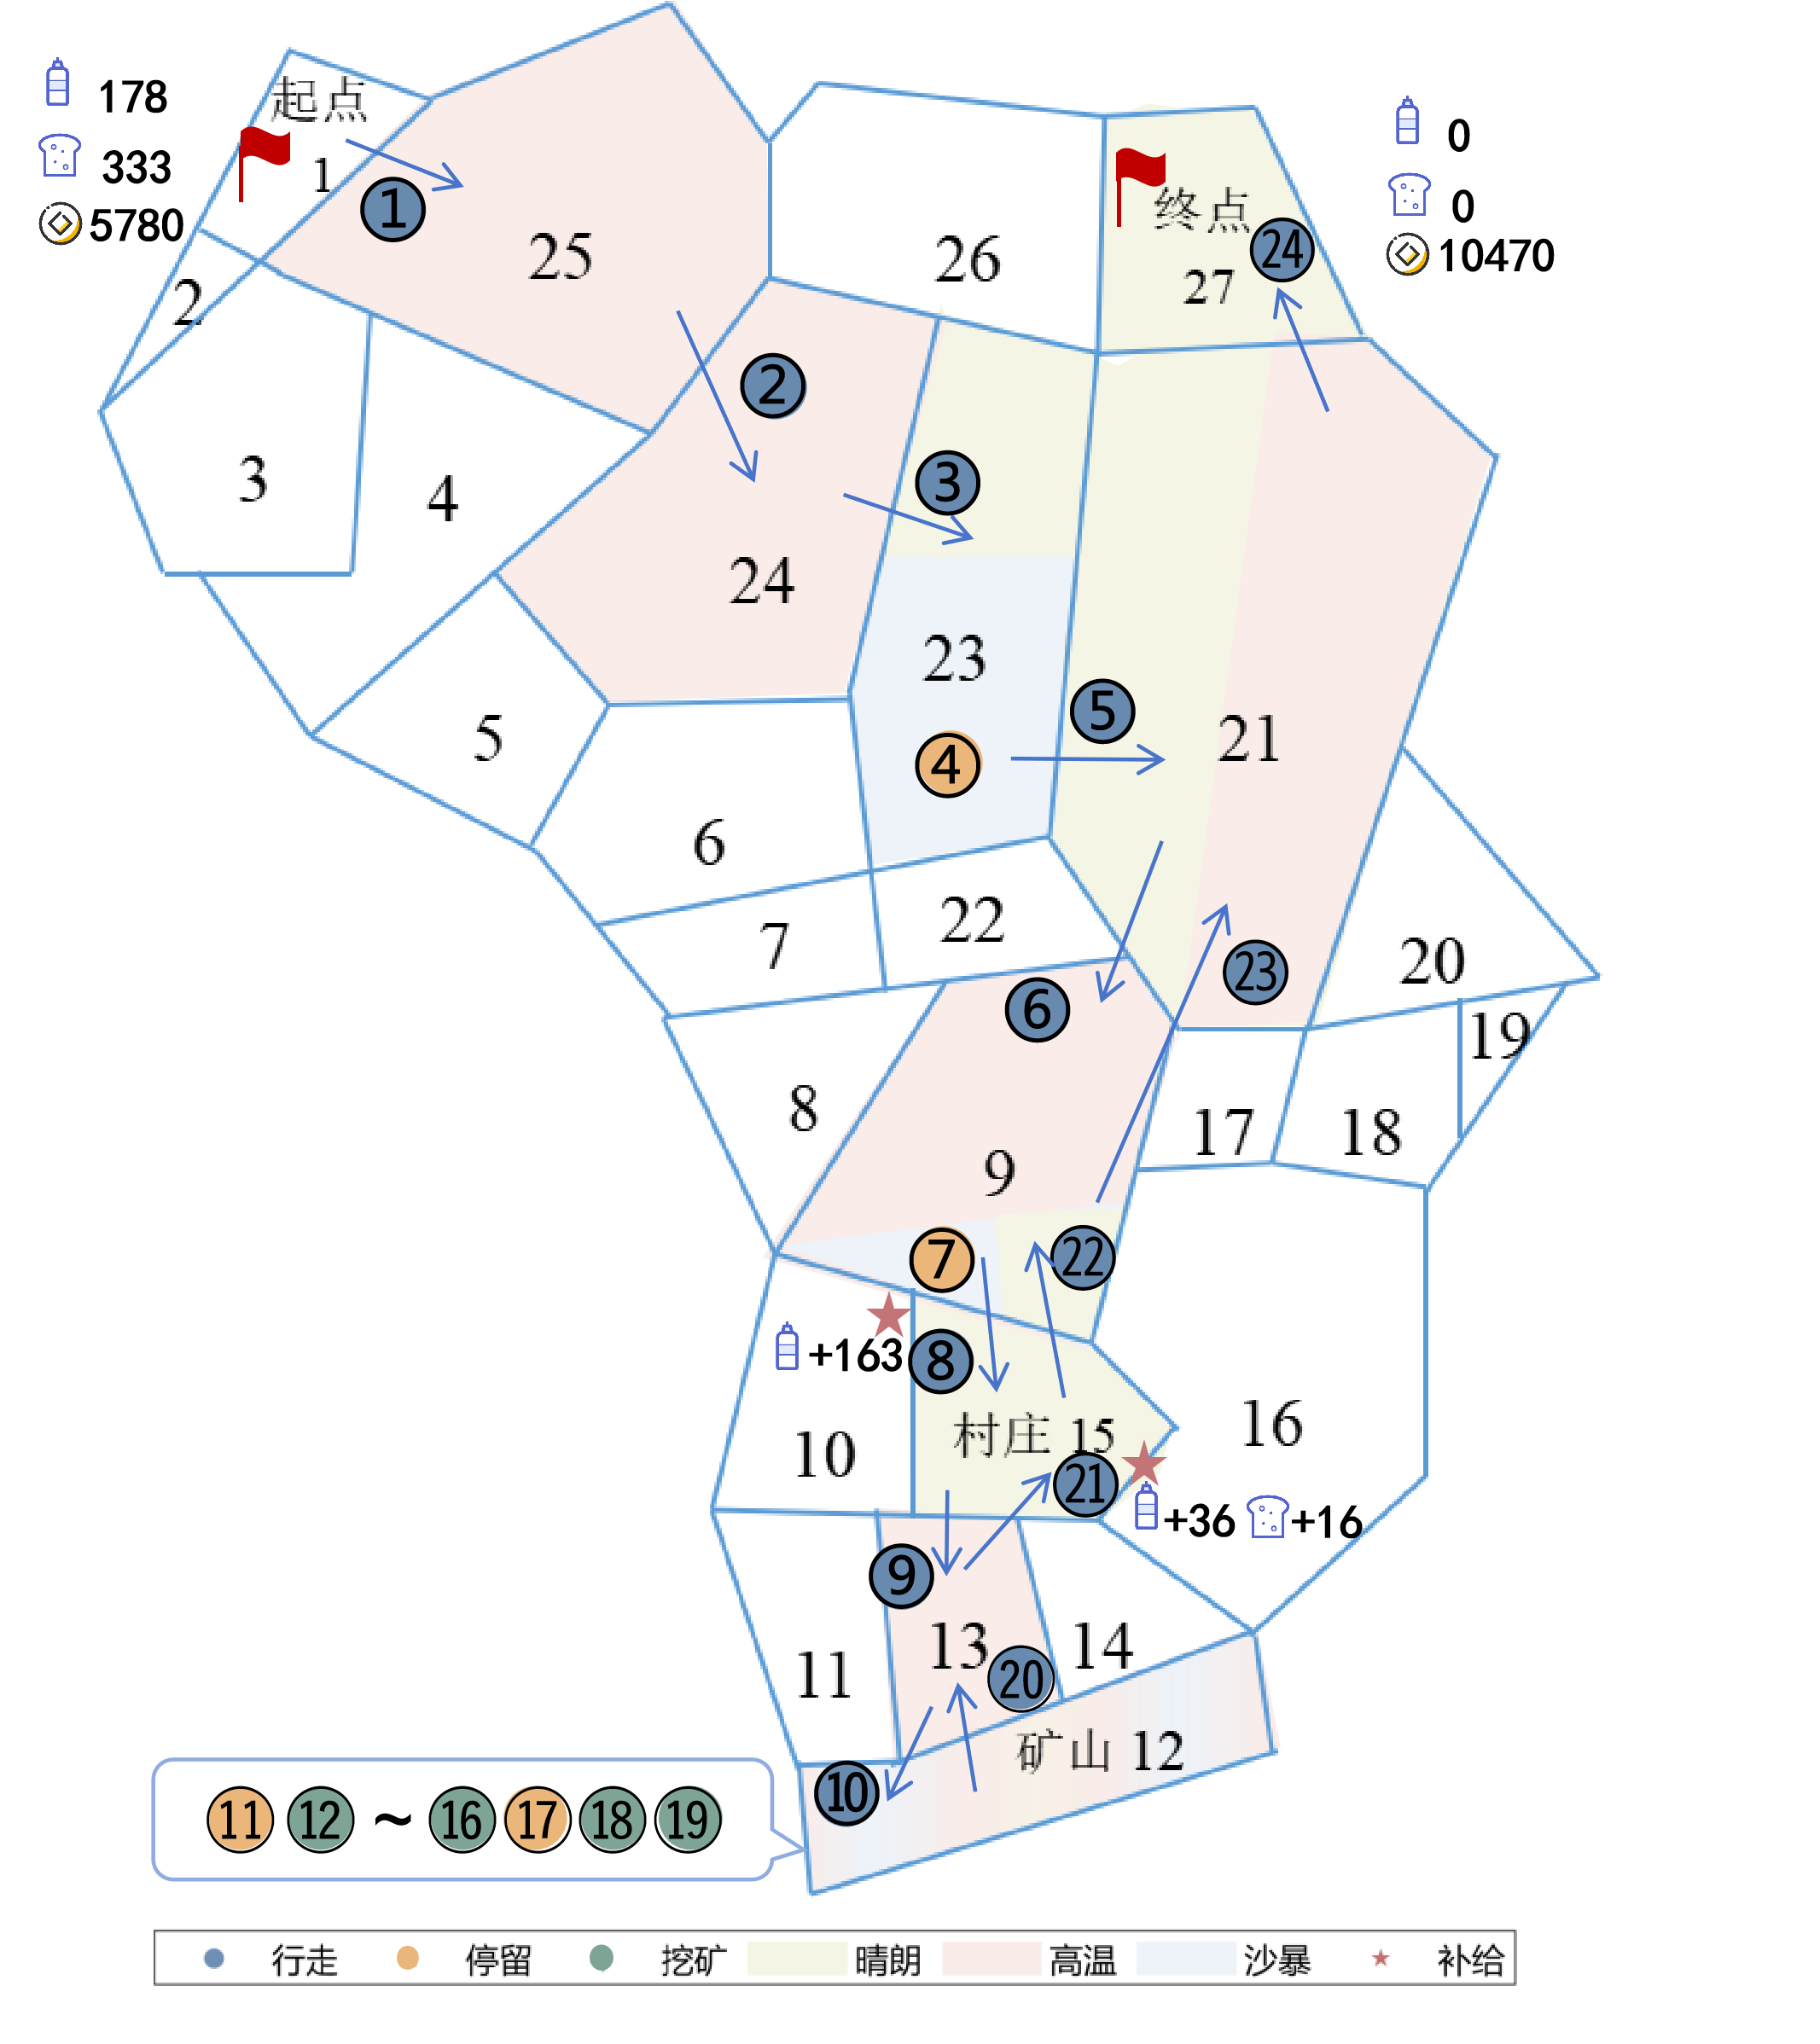
\includegraphics[width=0.5\textwidth]{fig_q1_route_level1.png}
    \caption{第一关最优行进路线}
    \label{fig:q1_route1}
\end{figure}

\textbf{第一关：}最优策略如图~\ref{fig:q1_route1}所示，详细策略如表~\ref{tab:q1_daily1}（见附录），最优终端财富为 10470 元，第 24 天到达终点。第 0 天购买 178 箱水和 333 箱食物，后续分别于第 8 天和第 21 天在村庄补给。策略包含两段挖矿阶段，共挖矿 7 天，并在第 17 天沙暴日选择停留，最终水和食物均恰好耗尽。

\begin{figure}[H]
    \centering
    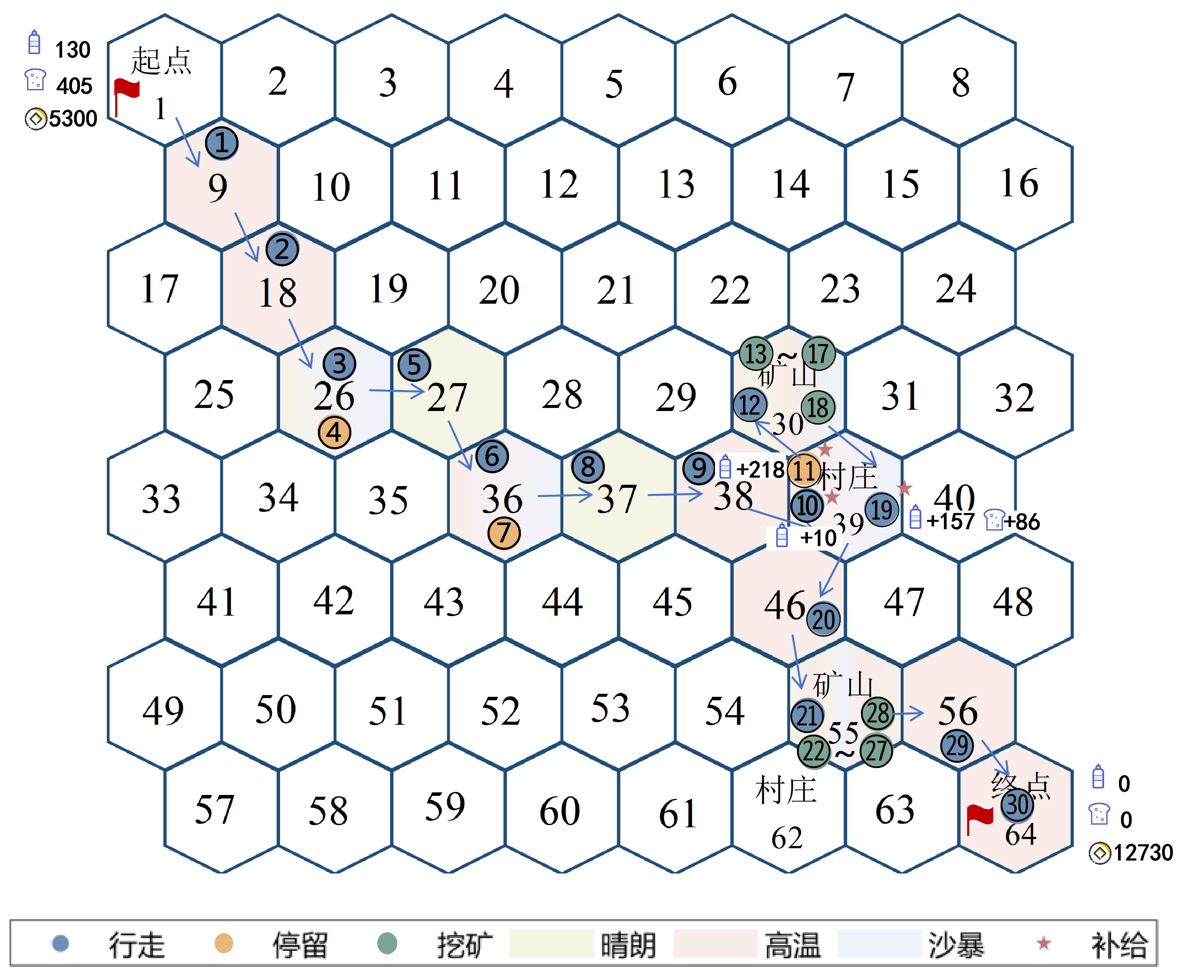
\includegraphics[width=0.5\textwidth]{fig_q1_route_level2.png}
    \caption{第二关最优行进路线}
    \label{fig:q1_route2}
\end{figure}

\textbf{第二关：}最优策略如图~\ref{fig:q1_route2}所示，详细策略如表~\ref{tab:q1_daily2}（见附录），最优终端财富为 12730 元，第 30 天到达终点。第 0 天购买 130 箱水和 405 箱食物，途中在村庄进行 3 次补给，并分两阶段挖矿共 13 天。相比第一关，增加的挖矿收益有效覆盖了补给成本，使终端财富提高 2260 元。

\begin{figure}[H]
    \centering
    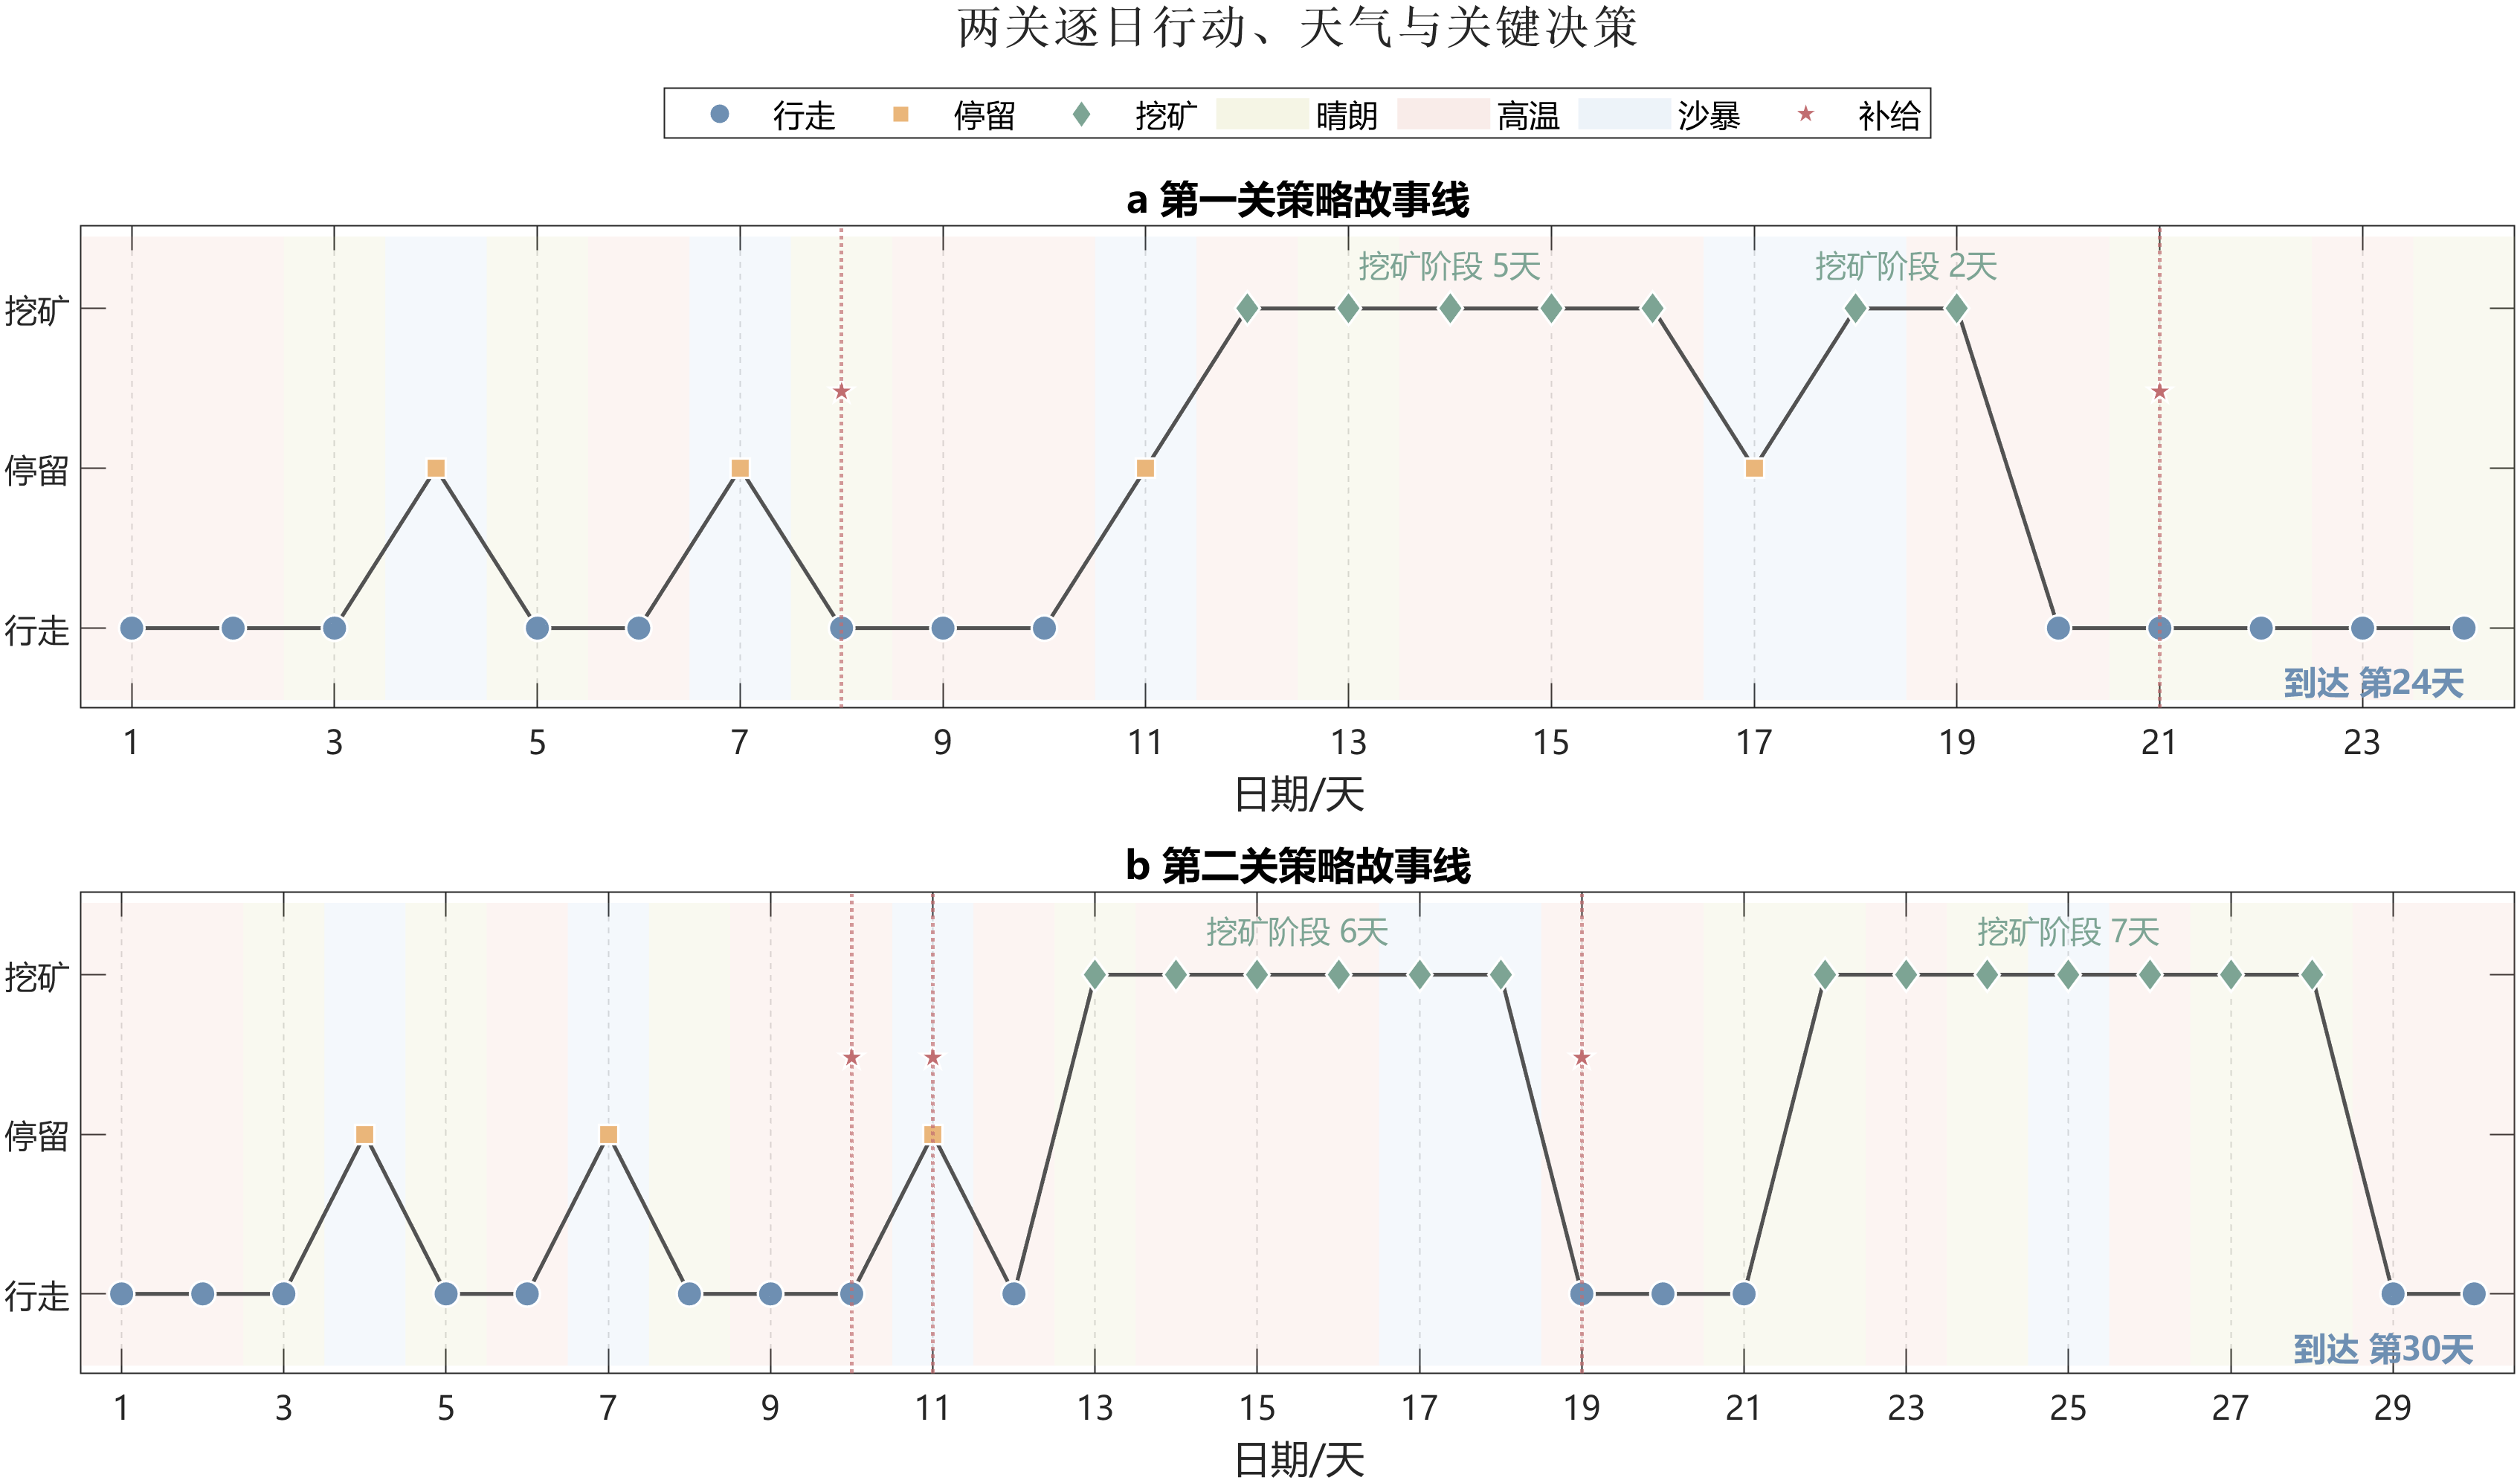
\includegraphics[width=0.98\textwidth]{fig_q1_strategy_storyboard.png}
    \caption{两关逐日行动、天气与关键决策}
    \label{fig:q1_storyboard}
\end{figure}

\begin{figure}[H]
    \centering
    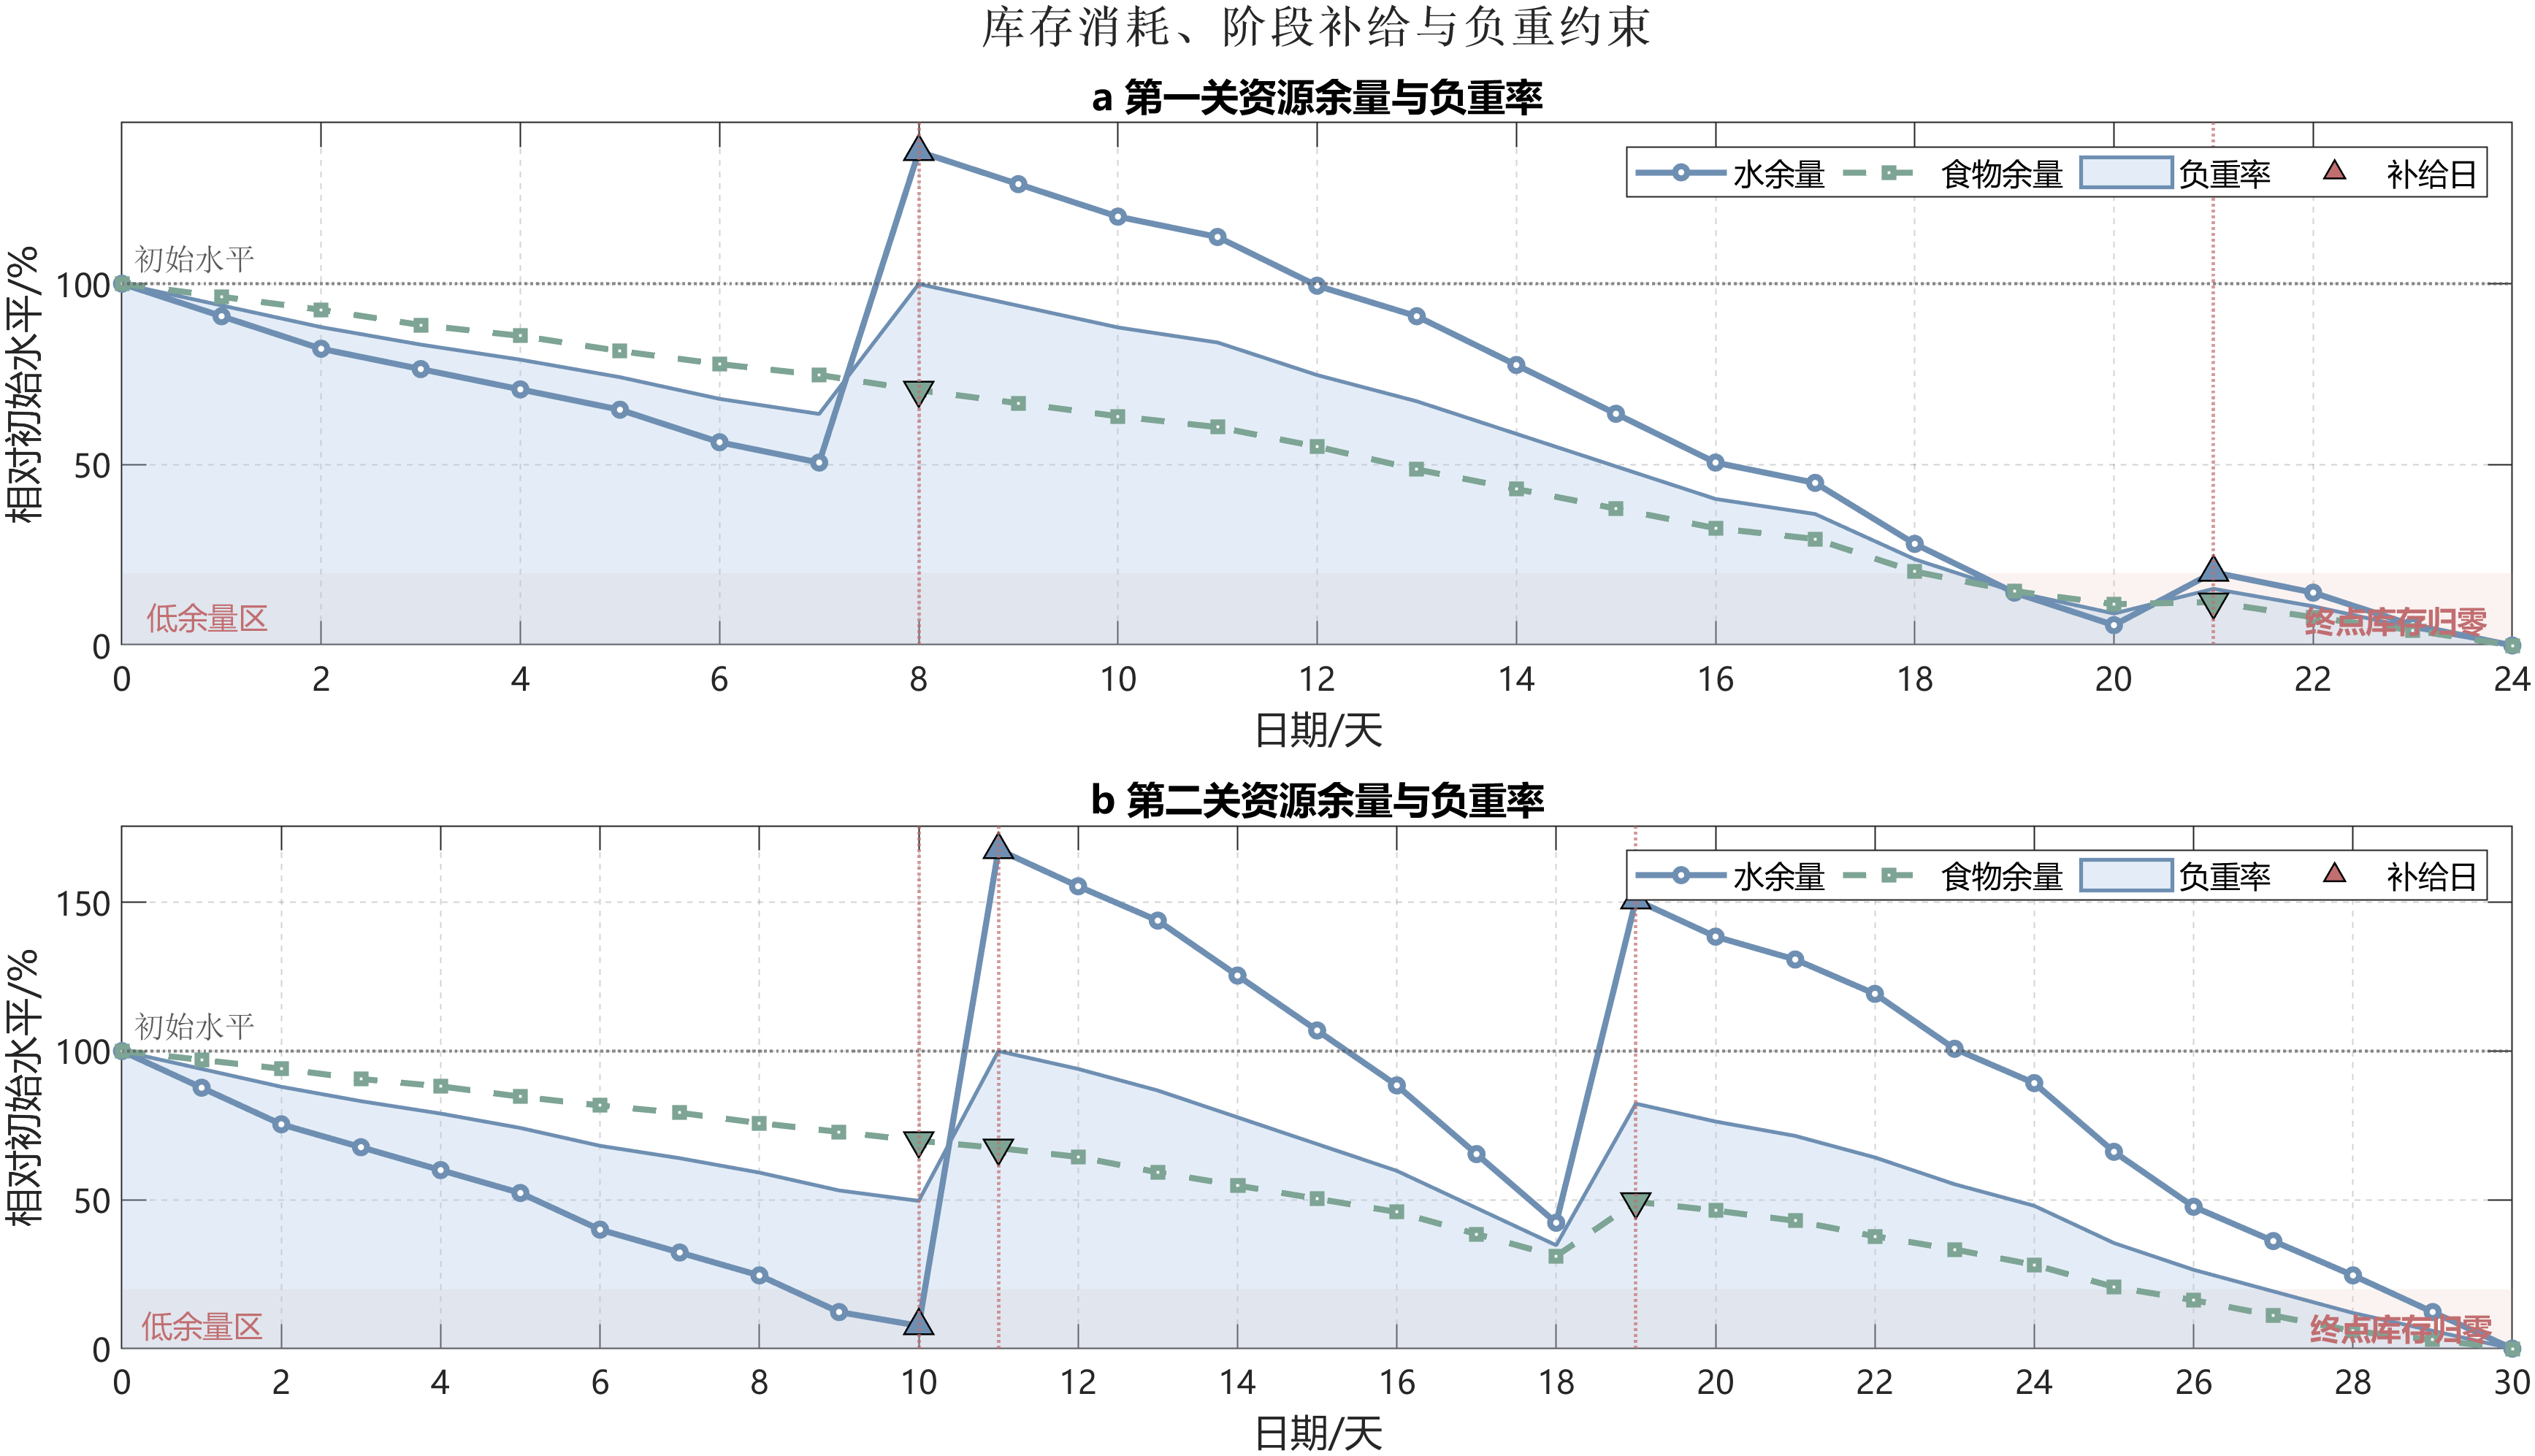
\includegraphics[width=0.98\textwidth]{fig_q1_resource_ribbon.png}
    \caption{库存消耗、阶段补给与负重约束}
    \label{fig:q1_resource}
\end{figure}
由图~\ref{fig:q1_storyboard} 可见，两关均在天气约束下完成行走、停留和挖矿状态的逐日切换，补给节点与后续挖矿或末段行走紧密衔接。从资源约束图（图~\ref{fig:q1_resource}）看，两关第 0 天负重率均为 100\%；补给日库存出现跃升后持续消耗，终点精确归零。第一关第 8 天补水后水余量超过初始水平，说明补给量精确匹配后续挖矿与移动的消耗需求。

\begin{figure}[H]
    \centering
    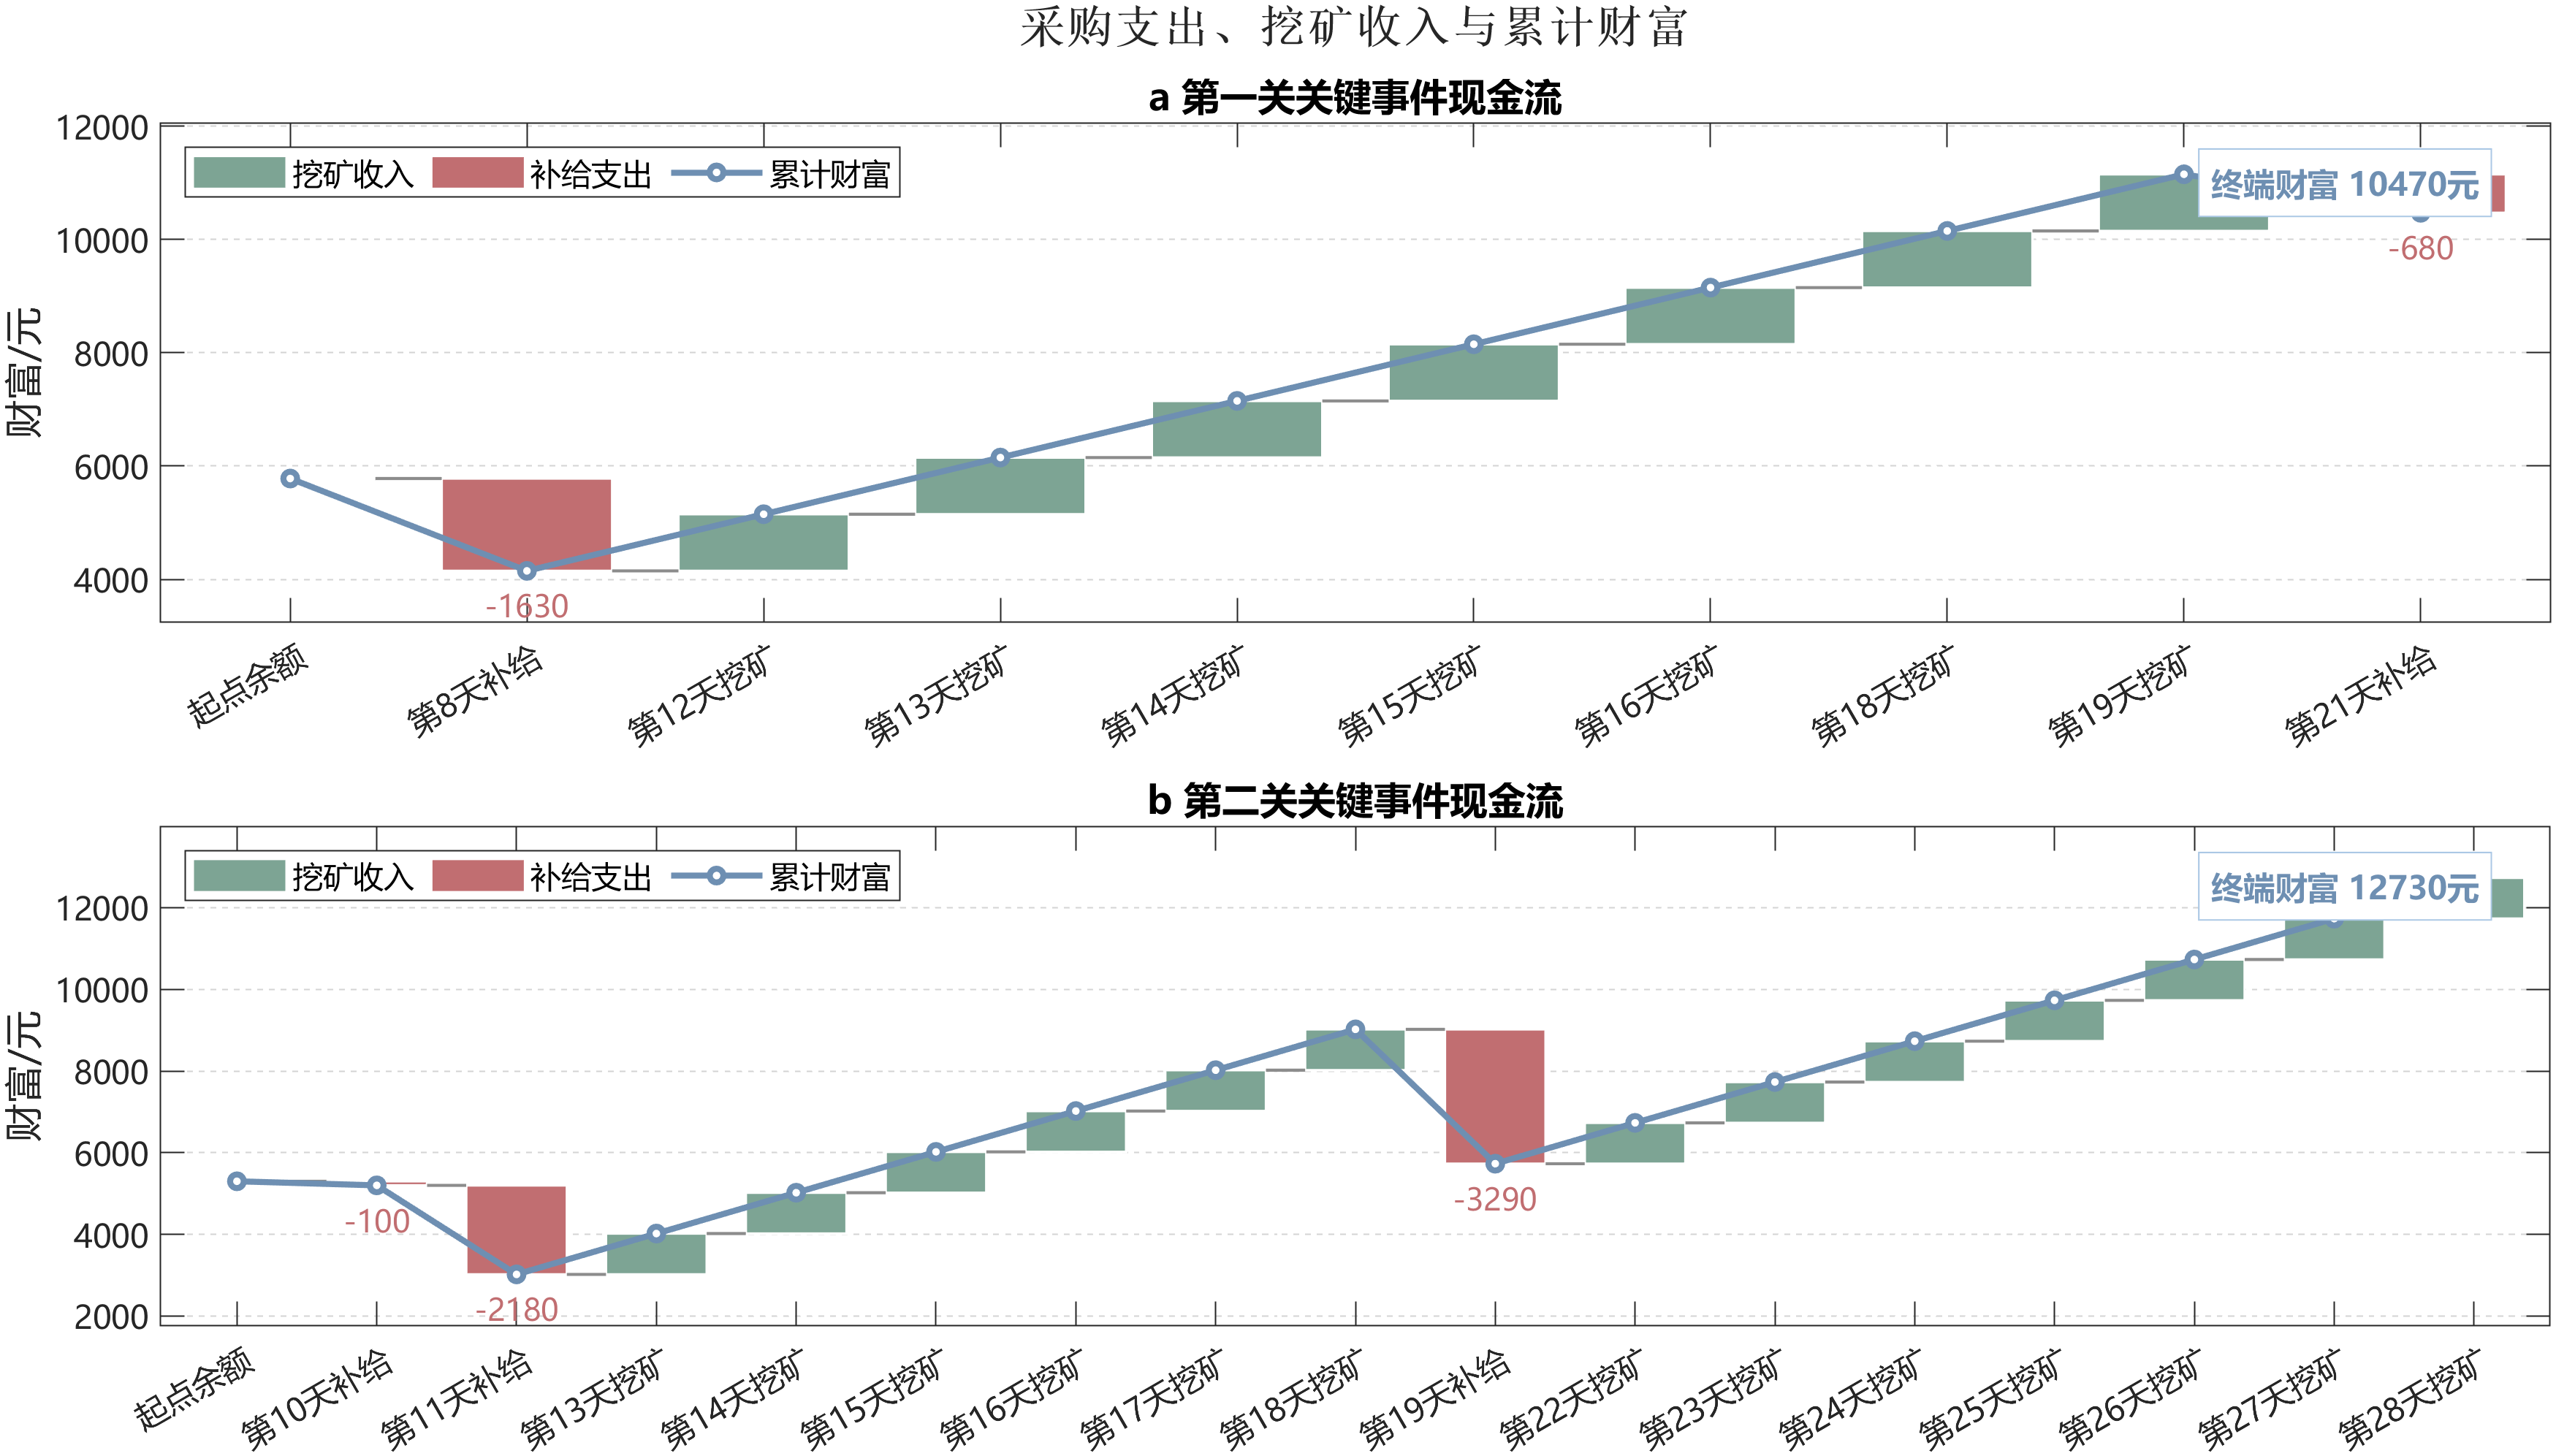
\includegraphics[width=0.98\textwidth]{fig_q1_cashflow_waterfall.png}
    \caption{采购支出、挖矿收入与累计财富}
    \label{fig:q1_cashflow}
\end{figure}

从现金流图（图~\ref{fig:q1_cashflow}）看，第一关两次补给分别支出 1630 元和 680 元，共 2310 元，7 个挖矿日各带来 1000 元收益，终端现金 10470 元。

两关的逐日最优决策（每日天气、行动、所在区域、补给量以及剩余资金/水量/食物量）详见附录表~\ref{tab:q1_daily1} 与表~\ref{tab:q1_daily2}。

由表~\ref{tab:q1_daily1} 可见，第一关第 1--8 天沿节点序列 $1\to25\to24\to23\to21\to9$ 到达村庄 15（第 4、7 天因沙暴停留），第 8 天一次补水 163 箱后行至矿山 12，并于第 12--19 天连续挖矿 7 天（第 17 天沙暴休息），累计增收 7000 元；第 21 天回村补给 36 箱水、16 箱食物，第 24 天到达终点，水和食物恰好耗尽。表~\ref{tab:q1_daily2} 表明第二关采用“双阶段挖矿”策略：第 10--11 天在村庄 39 共补水 228 箱，支撑第 13--18 天在矿山 30 连续挖矿 6 天；第 19 天再次补给 157 箱水、86 箱食物后，于第 22--28 天在矿山 55 连续挖矿 7 天，两段合计挖矿 13 天、增收 13000 元，最终第 30 天到达终点。
\subsubsection{最优性验证}

为保障求解结果的可信度，本文采用独立于求解器的验证机制。首先，独立 checker 从第 0 天逐日重算，对邻接关系、天气约束、动作合法性、村庄采购、资源非负、现金非负、负重上限和终止条件等九类规则逐一审计，两关均未发现违规。其次，通过关闭全部剪枝重新求解并与开启剪枝的结果对照，证明三种剪枝策略均不改变全局最优解。最后，针对终点吸收规则进行回归测试：将终点状态扩展到下一天的逻辑关闭后，终端财富保持 10470 元与 12730 元不变，确认终点吸收处理正确。

\subsubsection{灵敏性分析}

采用单因素离散扰动法，每次只改变一个参数并重新求解完整整数模型，而非在基准解附近做线性外推。各参数扰动下的最优财富与策略结构变化如表~\ref{tab:q1_sens} 所示，整体响应排序见图~\ref{fig:q1_sensitivity}。

\begin{figure}[H]
    \centering
    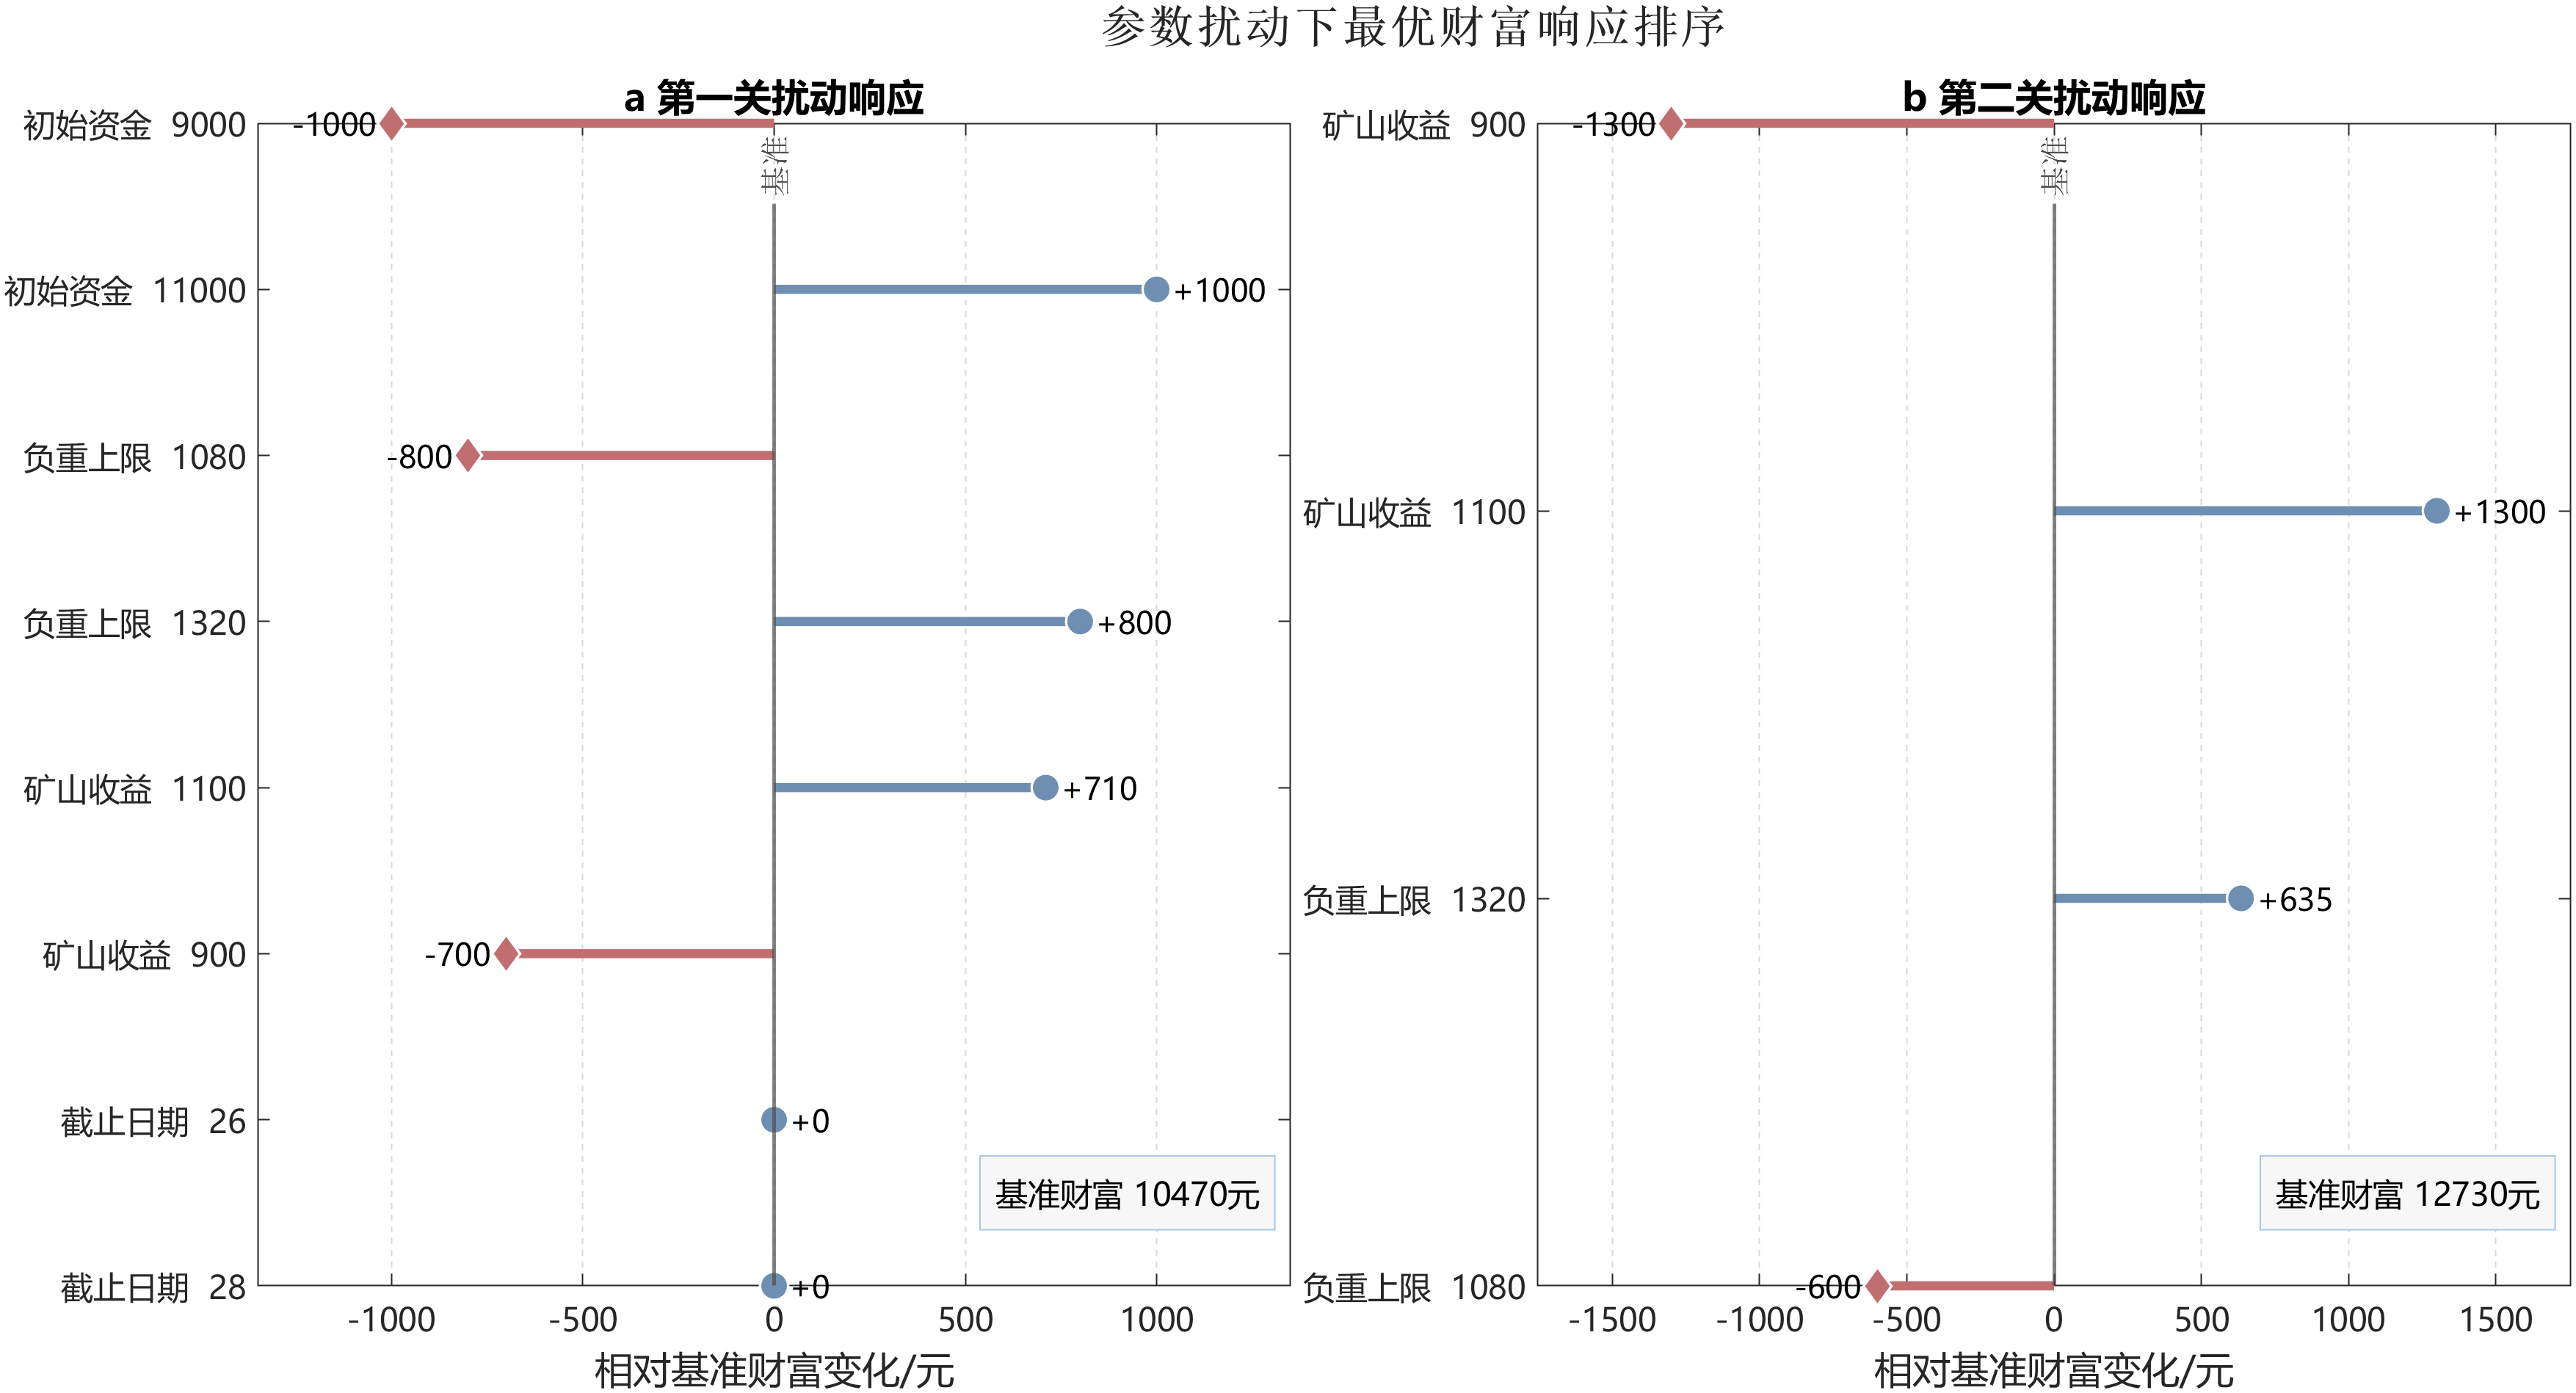
\includegraphics[width=0.98\textwidth]{fig_q1_sensitivity_lollipop.png}
    \caption{参数扰动下最优财富响应排序}
    \label{fig:q1_sensitivity}
\end{figure}

{
\begin{longtable}{llcccccc}
    \caption{第一问参数扰动下的最优财富与策略结构}
    \label{tab:q1_sens} \\
    \toprule
    关卡 & 扰动参数 & 参数值 & 最优财富/元 & 到达日 & 挖矿天数 & 补给次数 & 初始水/食物(箱) \\
    \midrule
    \endfirsthead

    \multicolumn{8}{c}{表~\ref{tab:q1_sens}（续）} \\
    \toprule
    关卡 & 扰动参数 & 参数值 & 最优财富/元 & 到达日 & 挖矿天数 & 补给次数 & 初始水/食物(箱) \\
    \midrule
    \endhead

    \midrule
    \multicolumn{8}{r}{续下页} \\
    \endfoot

    \bottomrule
    \endlastfoot

    第一关 & 基准 & 基准 & 10470 & 24 & 7 & 2 & 178/333 \\
    第一关 & 负重上限 & 1080 & 9670 & 24 & 6 & 2 & 158/303 \\
    第一关 & 负重上限 & 1320 & 11270 & 24 & 8 & 2 & 198/363 \\
    第一关 & 矿山收益 & 900 & 9770 & 24 & 7 & 2 & 178/333 \\
    第一关 & 矿山收益 & 1100 & 11180 & 28 & 8 & 3 & 162/357 \\
    第一关 & 初始资金 & 9000 & 9470 & 24 & 7 & 2 & 178/333 \\
    第一关 & 初始资金 & 11000 & 11470 & 24 & 7 & 2 & 178/333 \\
    第一关 & 截止日期 & 26 & 10470 & 24 & 7 & 2 & 178/333 \\
    第一关 & 截止日期 & 28 & 10470 & 24 & 7 & 2 & 178/333 \\

    \midrule

    第二关 & 基准 & 基准 & 12730 & 30 & 13 & 3 & 130/405 \\
    第二关 & 负重上限 & 1080 & 12130 & 30 & 13 & 3 & 130/345 \\
    第二关 & 负重上限 & 1320 & 13365 & 30 & 14 & 1 & 247/289 \\
    第二关 & 矿山收益 & 900 & 11430 & 30 & 13 & 3 & 130/405 \\
    第二关 & 矿山收益 & 1100 & 14030 & 30 & 13 & 3 & 130/405 \\
    
\end{longtable}
}

结果表明：负重上限对两关均呈显著正向影响。由表~\ref{tab:q1_sens} 可知，第一关负重由 1200 kg 下调至 1080 kg 时，最优财富由 10470 元降至 9670 元；上调至 1320 kg 后增至 11270 元。第二关相应由 12130 元上升到 13365 元。这说明容量不仅减少补给成本，还改变可持续挖矿天数和跨补给点运输能力。

矿山收益的影响近似分段线性，斜率由最优挖矿天数决定。第一关收益从 1000 元降至 900 元时，最优财富降至 9770 元；升至 1100 元时增至 11180 元。第二关分别为 11430 元和 14030 元，变化幅度更大——由图~\ref{fig:q1_sensitivity} 可见第二关对矿山收益最敏感，财富变化达正负 1300 元，原因是基准策略共挖矿 13 天，收益对总财富的传导系数更高。

第一关中，初始资金由 9000 元增至 11000 元时，最优财富同步增加，说明该区间内最优路线和采购结构基本稳定。截止日期调整至 26 天或 28 天时，最优财富仍为 10470 元，主要由于基准策略第 24 天已到达终点，具有充足的时间裕度；相比之下，第二关第 30 天才到达终点，时间约束更为显著。
\begin{figure}[H]
    \centering
    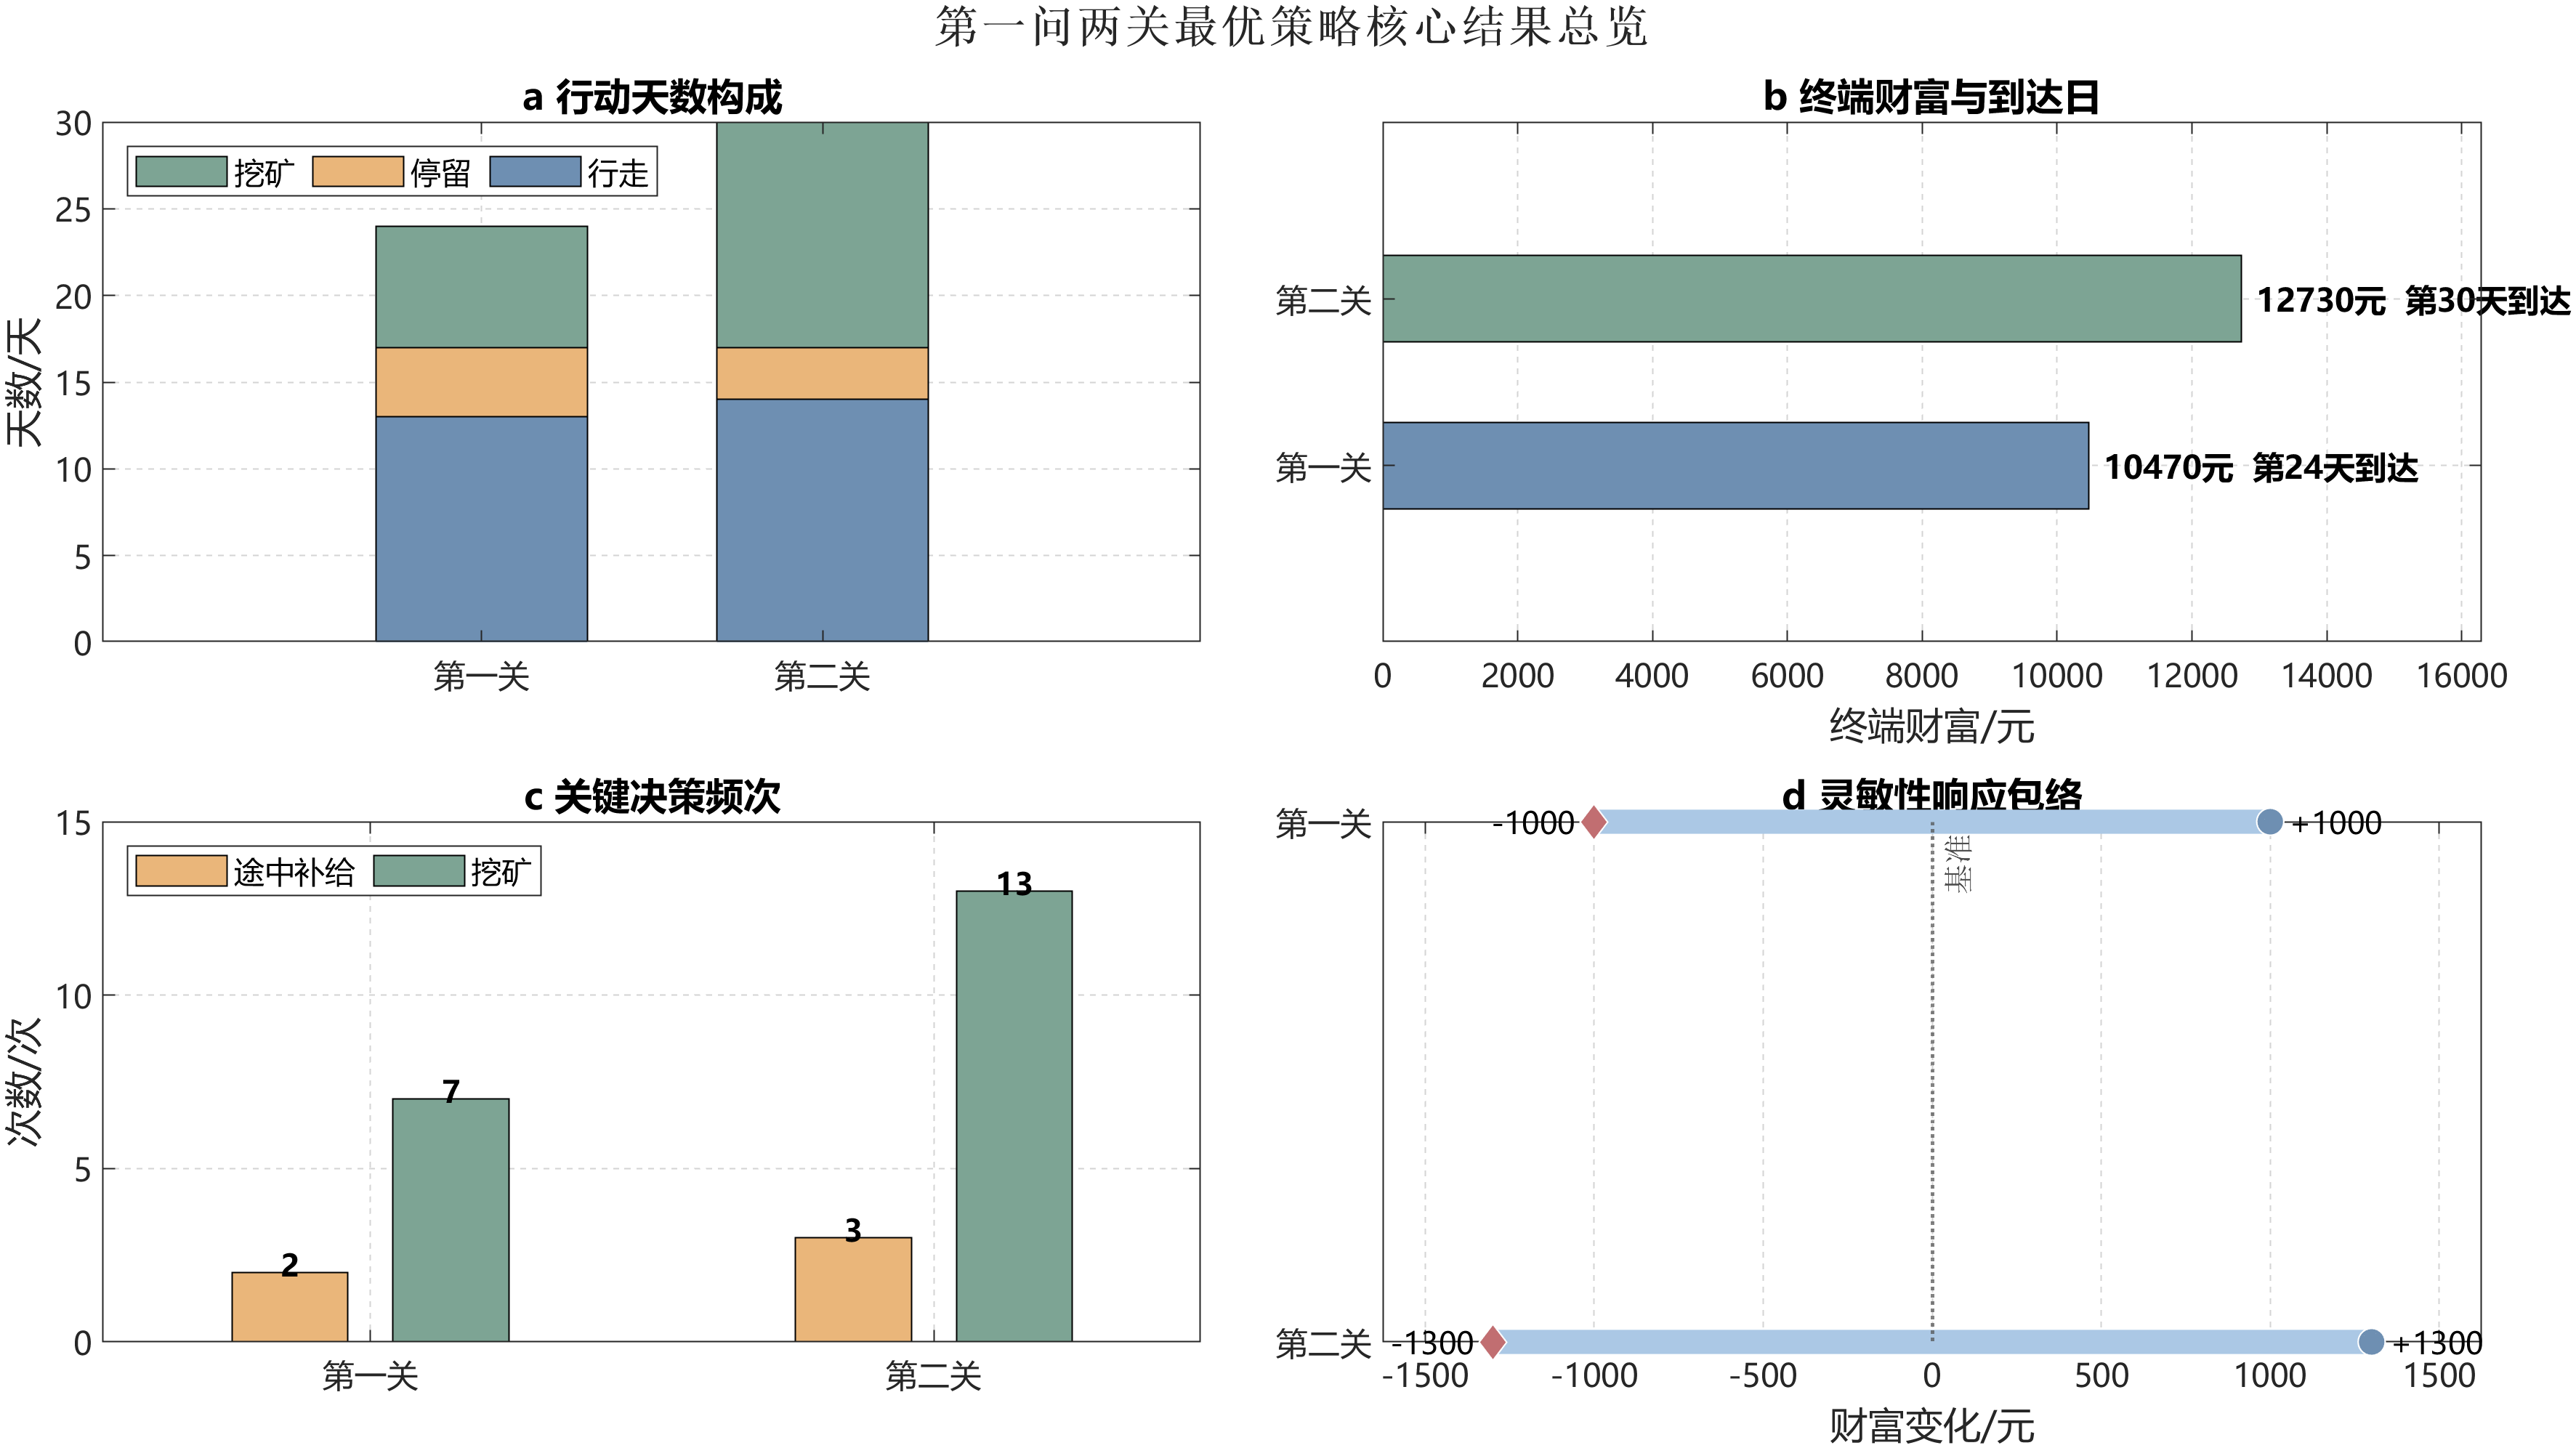
\includegraphics[width=0.98\textwidth]{fig_q1_strategy_dashboard.png}
    \caption{第一问两关最优策略核心结果总览}
    \label{fig:q1_dashboard}
\end{figure}

图~\ref{fig:q1_dashboard} 的总览仪表盘汇总了两关的核心指标：第二关比第一关多 6 天、多 6 个挖矿日和 1 次途中补给，最终财富高 2260 元，但灵敏性响应范围也更宽。

\subsubsection{问题一结论}

综合上述求解与验证，第一问得到以下结论：

\textbf{第一，}建立的有限期资源约束动态规划模型能够有效描述天气、行动、资源消耗、补给与收益之间的动态关系。两关均获得全局最优解：\textbf{第一关终端财富为 10470 元，第 24 天到达；第二关终端财富为 12730 元，第 30 天到达。}剪枝策略及独立 checker 验证均表明所得结果具有可靠性。

\textbf{第二，}两关最优策略均呈现“起点采购—集中挖矿—村庄补给”的基本结构，通过合理安排挖矿与补给实现财富最大化；其中第二关利用多矿山、多村庄的路径结构获得了更高收益。

\textbf{第三，}灵敏性分析表明，矿山收益和负重上限对最优财富影响较明显；第一关截止日期具有一定时间裕度，而第二关到达日与截止日重合，时间约束更为紧张。该模型适用于天气完全已知条件下的离线最优策略制定。

\subsection{问题二模型建立与求解}

\subsubsection{不确定性结构}


第三关与第四关具有不同的不确定性结构，需分别处理。第三关明确未来10日内无沙暴，未来天气只能取晴朗(S)与高温(H)两种，完整情景数仅为$2^{10}=1024$，可穷举全部情景直接求解鲁棒最优。第四关仅说明"30日内沙暴较少"，既未给出沙暴概率也未给出最多沙暴天数，任何将其改写成固定概率或固定天数上限的做法都引入了题面之外的假设。为此本文不预设沙暴分布，而将沙暴天数保留为预算参数$\Gamma$，构造不确定集
\begin{equation}
\Omega_4(\Gamma)=\bigl\{\omega\in\{S,H,X\}^{30} : \textstyle\sum_{t=1}^{30}\mathbb{I}(\omega_t=X)\le \Gamma\bigr\}
\label{eq:q2_omega4}
\end{equation}
并以题内30日样本中的6个沙暴日作为数据锚定，扫描$\Gamma=0,1,\dots,6$，得到"$\Gamma$—策略—财富"稳健前沿，而不是锁死某个单一概率。


\subsubsection{自适应鲁棒动态规划主模型}

\begin{enumerate}
    \item  \textbf{状态与策略}
    
    设第$t$日观察到当天气候$\omega_t$后玩家状态为
\begin{equation}
s_t=(i_t,\ W_t,\ F_t,\ C_t)
\label{eq:q2_state}
\end{equation}
其中$i_t$为日末所在区域，$W_t$、$F_t$为水和食物箱数，$C_t$为现金；第四关额外记录已发生沙暴数$q_t$或剩余沙暴预算$b_t=\Gamma-q_t$。在线策略是从可见历史到动作的映射：
\begin{equation}
a_t=\pi_t(h_t,\omega_t),\qquad h_t=(s_0,\omega_1,a_1,\dots,s_t)
\label{eq:q2_policy}
\end{equation}
非前视约束要求：若两条天气路径在第$t$日前拥有完全相同的可见历史与当天天气，则必须给出相同动作，即
\begin{equation}
h_t(\omega)=h_t(\omega')\ \Rightarrow\ \pi_t(\omega)=\pi_t(\omega')
\label{eq:q2_nonanticip}
\end{equation}
由此，求解器在任何情况下都无法"偷看"未来天气，策略表随状态反馈逐日生成。

    \item  \textbf{动作集合与状态转移}
    
    每天从合法动作集$A(s,\omega)$中选择动作。停留、行走、挖矿的消耗倍率分别为1、2、3；沙暴日禁止移动，但允许停留与矿山挖矿；到达矿山当日不能挖矿；购买仅在第0日起点（基准价）与村庄（基准价的2倍）进行。设天气$\omega_t$下的基础消耗为$c_w(\omega_t)$、$c_f(\omega_t)$，则
\begin{equation}
W_{t+1}=W_t+b^W_t-\kappa(a_t)c_w(\omega_t),\qquad
F_{t+1}=F_t+b^F_t-\kappa(a_t)c_f(\omega_t)
\label{eq:q2_resource}
\end{equation}
\begin{equation}
C_{t+1}=C_t-\beta\,p_w b^W_t-\beta\,p_f b^F_t+R\cdot\mathbb{I}(a_t=\text{挖矿})
\label{eq:q2_cash}
\end{equation}
其中$\beta=1$（起点）或$\beta=2$（村庄），$R$为基础挖矿收益，$b^W_t$、$b^F_t$为当日购买量。所有状态须满足资源非负、现金非负与负重约束
\begin{equation}
W_t\ge 0,\quad F_t\ge 0,\quad C_t\ge 0,\quad m_w W_t+m_f F_t\le M
\label{eq:q2_con}
\end{equation}

    为避免"先透支再到村庄补给"的非法行为，从非村庄节点移动至村庄当日的消耗由移动前库存满足，购买只作用于后续状态。

    \item  \textbf{终端目标与字典序目标}
    
    到达终点后剩余资源按基准价一半回收，任一天$\tau\le T$到达终点时的终端财富为
\begin{equation}
Z(\tau)=C_\tau+0.5\,p_w W_\tau+0.5\,p_f F_\tau
\label{eq:q2_terminal}
\end{equation}
第三关在无合法概率分布的前提下采用自适应鲁棒最大最小目标
\begin{equation}
\max_{\pi\in\Pi_{\text{NA}}}\ \min_{\omega\in\Omega_3} Z(\pi,\omega)
\label{eq:q2_obj3}
\end{equation}
第四关对给定压力等级$\Gamma$采用
\begin{equation}
\max_{\pi\in\Pi_{\text{NA}}}\ \min_{\omega\in\Omega_4(\Gamma)} Z(\pi,\omega)
\label{eq:q2_obj4}
\end{equation}
其中$\Pi_{\text{NA}}$为非前视策略集合。若多个策略最坏终端财富相同，则以名义Markov模型下的期望终端财富作第二级判别，形成字典序目标
\begin{equation}
\max_{\pi}\ \Bigl(\min_{\omega\in\Omega} Z(\pi,\omega),\ \ \mathbb{E}_{\hat{P}}\bigl[Z(\pi,\omega)\bigr]\Bigr)
\label{eq:q2_lex}
\end{equation}

    \item  \textbf{鲁棒Bellman递推}
    
    第三关的鲁棒Bellman递推为
\begin{equation}
V_t(s,\omega)=\max_{a\in A(s,\omega)}\ \min_{\omega'\in\{S,H\}}\ V_{t+1}\bigl(T(s,a,\omega),\omega'\bigr)
\label{eq:q2_bellman3}
\end{equation}
若当前位置已为终点则$V_t(s,\omega)=Z(s)$；若$t>T$仍未到达终点则该状态不可行。第四关将剩余沙暴预算纳入状态，递推为
\begin{equation}
V_t(s,\omega,b)=\max_{a\in A(s,\omega)}\ \min_{\omega'\in W(b)}\ V_{t+1}\bigl(T(s,a,\omega),\omega',b-\mathbb{I}(\omega'=X)\bigr)
\label{eq:q2_bellman4}
\end{equation}
\begin{equation}
W(b)=\{S,H,X\}\ (b>0),\qquad W(0)=\{S,H\}
\label{eq:q2_budget}
\end{equation}
递推所得是一张随状态变化的策略表，而非提前写死的路线。
\end{enumerate}

\subsubsection{辅助模型：经验Markov天气模型与名义MDP}

题内第一、二关提供同一条30日完整天气序列，这是题目内部唯一明确的"历史天气信息"。按S、H、X编码后晴朗9天、高温15天、沙暴6天，相邻两日共29次转移，无平滑常数、无主观先验：
\begin{equation}
\hat{P}_4=\begin{bmatrix}2/9&5/9&2/9\\5/14&6/14&3/14\\2/6&3/6&1/6\end{bmatrix}
\label{eq:q2_p4}
\end{equation}

第三关明确无沙暴，因此在非沙暴条件下重新归一化：
\begin{equation}
\hat{P}_3=\begin{bmatrix}2/7&5/7\\5/11&6/11\end{bmatrix}
\label{eq:q2_p3}
\end{equation}

名义Bellman评价为
\begin{equation}
\bar{V}_t(s,\omega)=\max_{a\in A(s,\omega)}\ \sum_{\omega'}\hat{P}_{\omega,\omega'}\,\bar{V}_{t+1}\bigl(T(s,a,\omega),\omega'\bigr)
\label{eq:q2_nominal}
\end{equation}
该模型只用于并列判别、名义期望与Monte Carlo仿真，不替代主模型的鲁棒结论。

\subsubsection{求解方法：非前视情景树MILP等价展开与状态剪枝}

第三关完整情景仅1024条，将鲁棒递推等价展开为以天气情景树为信息结构的MILP，并显式施加非前视约束。情景树以第0日为根，第$t$层每个节点对应一个截至第$t$日的天气历史前缀；根之后按S/H二叉展开，深度为10，共2046个非根节点、1024个终端叶子。每个树节点引入位置、资源、现金与动作变量，动作只依赖该节点对应的可见历史，从而由构造保证非前视性；最大最小目标经等价变换写入线性瓶颈约束。

第四关情景数$3^{30}$不可穷举，采用带剩余预算状态$b_t$的鲁棒递推，并配合三种不改变可行域的剪枝：\textbf{Pareto支配}：对相同$(t,\text{node},\omega,b)$下的两个状态$A=(W_A,F_A,C_A)$、$B=(W_B,F_B,C_B)$，若$W_A\ge W_B$、$F_A\ge F_B$、$C_A\ge C_B$且至少一项严格，则$B$未来不可能优于$A$，删除$B$。\textbf{时间下界}：剩余天数小于当前位置到终点的BFS最短步数时删除。\textbf{资源上界}：携带资源不超过"剩余天数$\times$最大单日消耗"，且始终受1200 kg负重约束。

\subsubsection{求解结果}

\textbf{第三关：}

\begin{table}[H]
    \centering
    \begin{tabular*}{\textwidth}{@{\extracolsep{\fill}}cc}
        \toprule
        指标 & 数值 \\
        \midrule
        初始采购（水,食）/箱 & 54, 54 \\
        初始采购后现金/元 & 9190 \\
        最坏终端财富/元 & 9190 \\
        名义Markov期望财富/元 & 9282.38 \\
        最坏情景 & HHHSSSSSSS \\
        到达日 & 3 \\
        情景总数 / 成功数 / 失败数 & 1024 / 1024 / 0 \\
        情景均值 / 5\%分位/元 & 9310 / 9190 \\
        Regret：均值 / 中位 / 最大/元 & 134.45 / 145 / 240 \\
        MILP规模 & 196419变量 / 94095约束 \\
        MIP间隙 & 0.0 \\
        求解时间/s & 60.22 \\
        \bottomrule
    \end{tabular*}
    \caption{第三关非前视鲁棒策略核心指标}
    \label{tab:q2_q3_core}
\end{table}

由表~\ref{tab:q2_q3_core} 可知，第三关鲁棒策略在第0日采购54箱水、54箱食物，第1--3日连续行走，于第3日到达终点。在所有1024种无沙暴天气序列上均成功到达，失败数为0。最坏情景为前三日连续高温HHHSSSSSSS，对应终端财富9190元；情景均值9310元、5\%分位9190元，与最坏值重合，说明最坏情形被多条序列同时触及。与完全信息Oracle相比，后悔值最小为0、中位数为145元、最大240元，即在1024种天气中，有一半情景因不预知未来天气仅损失不超过145元，表明该策略具有很强的近优性。

\begin{figure}[H]
    \centering
    \begin{subfigure}[t]{0.32\textwidth}
        \centering
        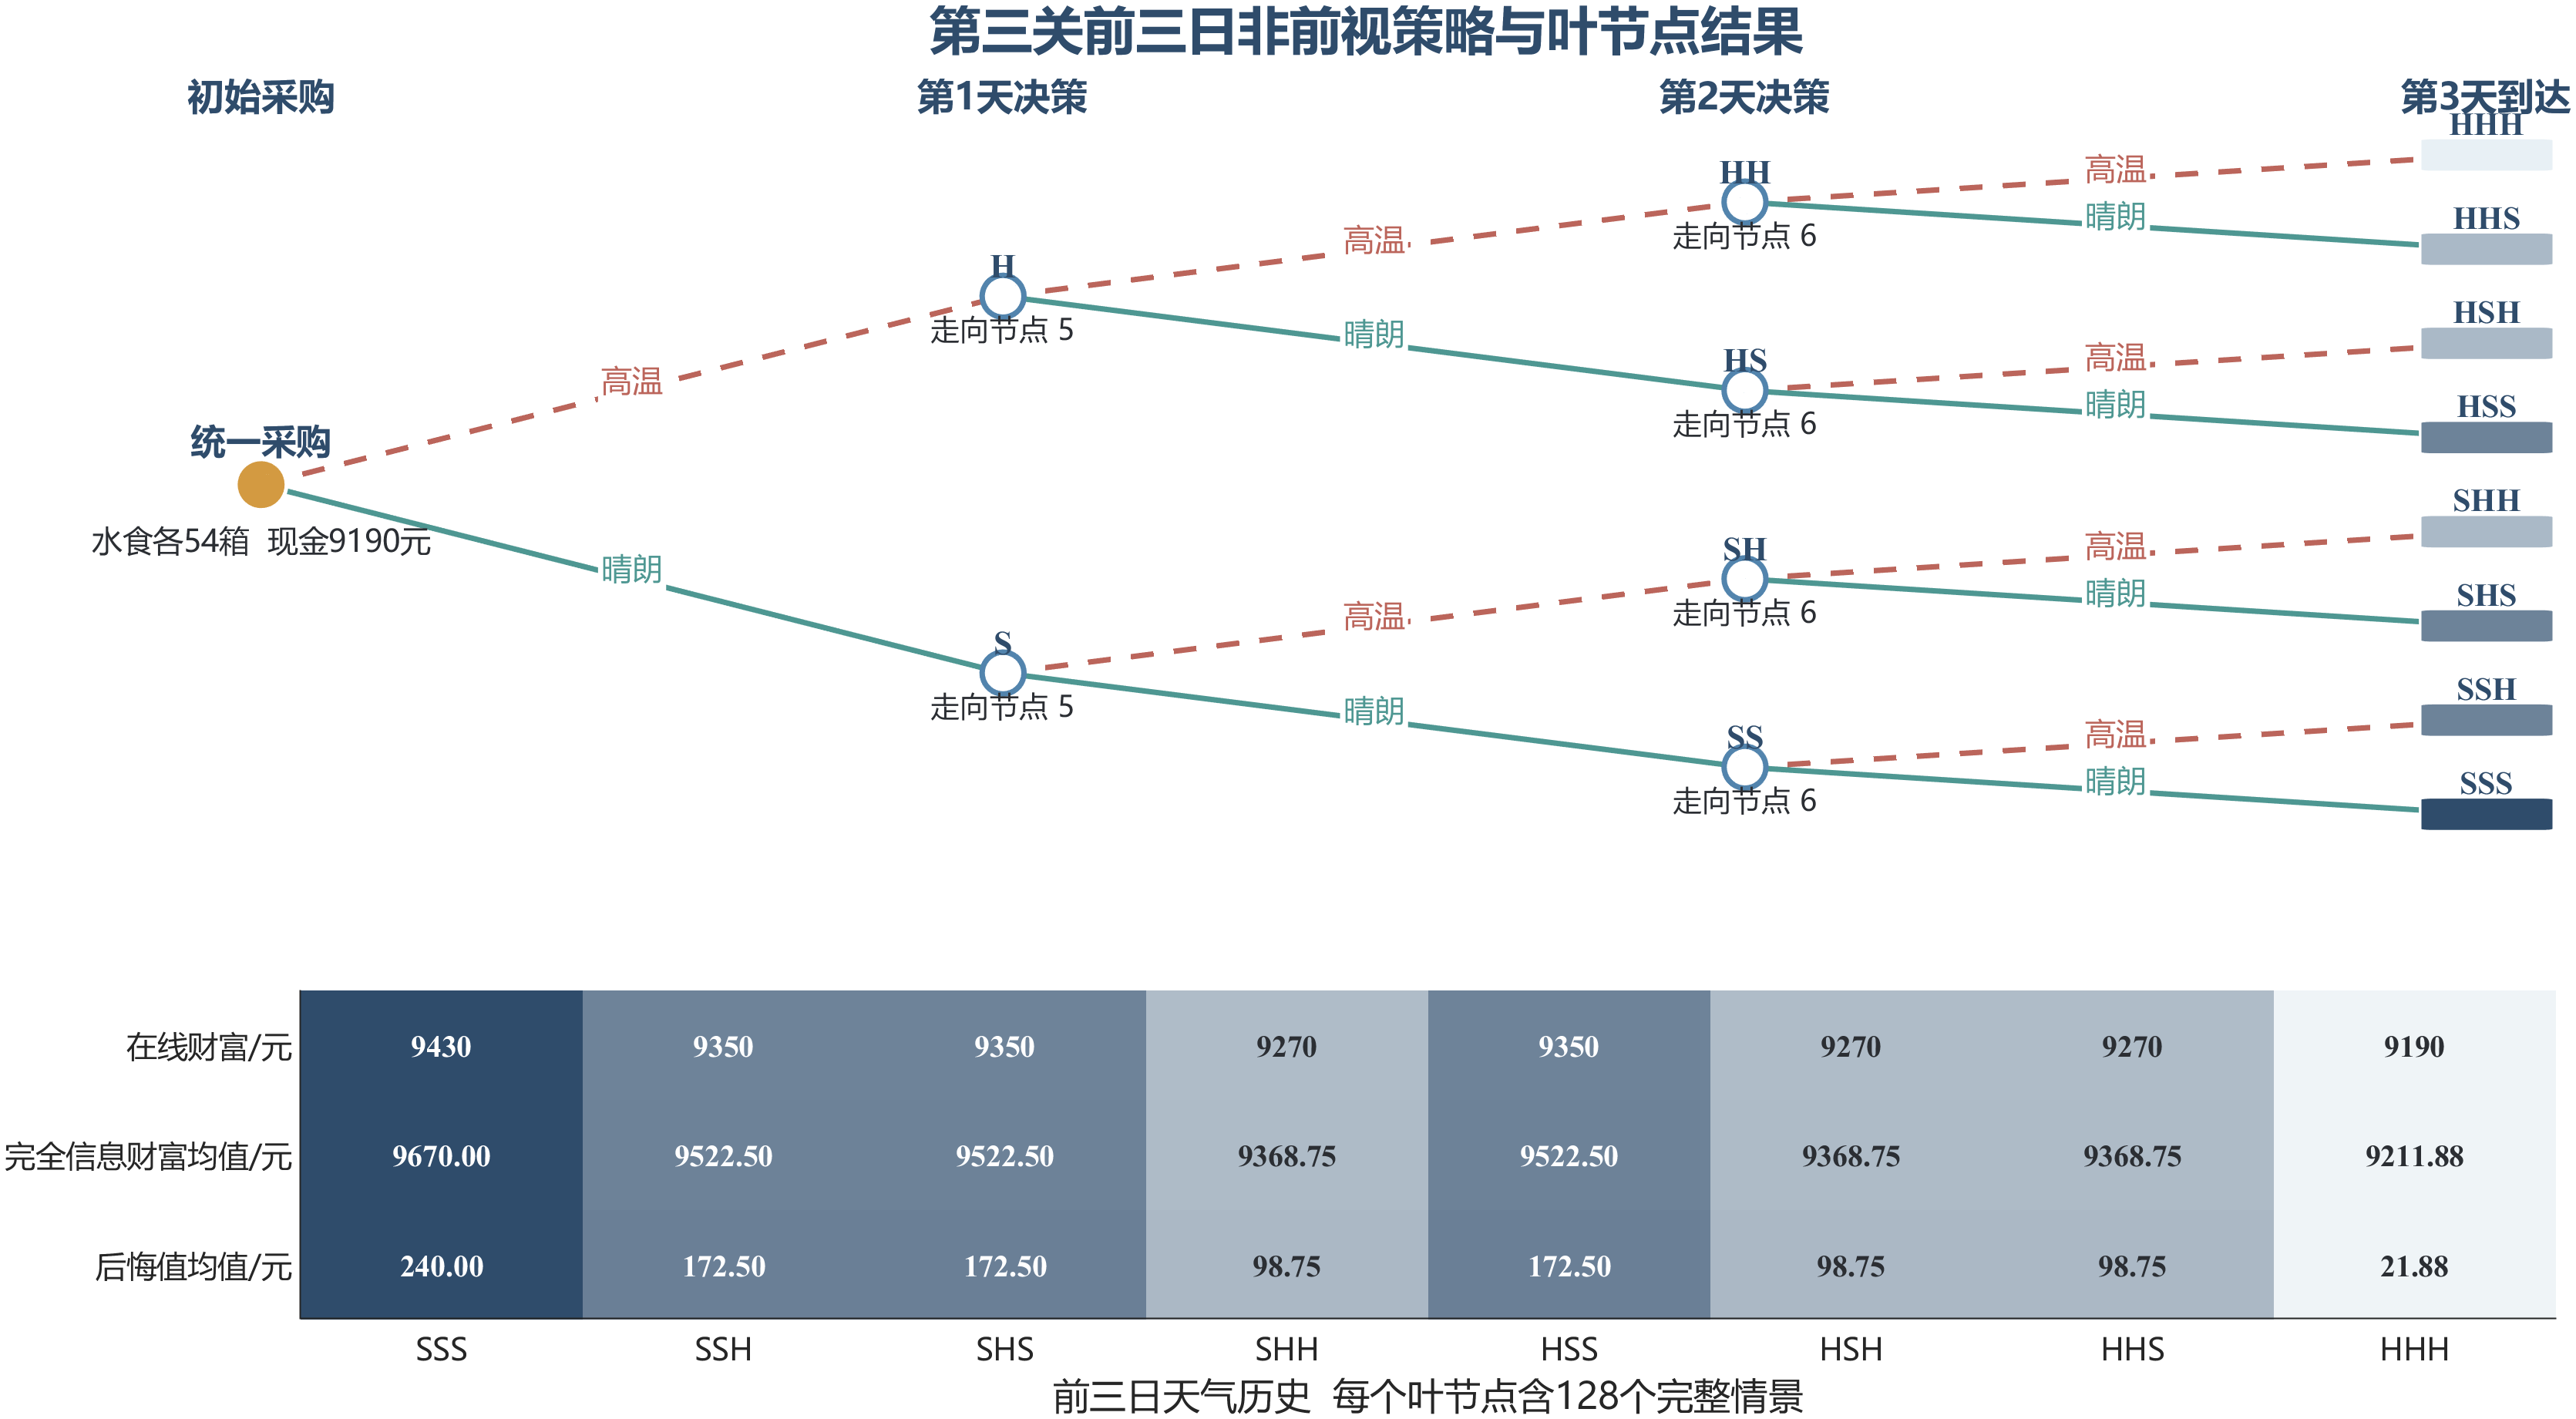
\includegraphics[width=\linewidth]{fig_q2_policy_tree.png}
        \caption{前三日非前视策略与叶节点结果}
    \end{subfigure}\hfill
    \begin{subfigure}[t]{0.32\textwidth}
        \centering
        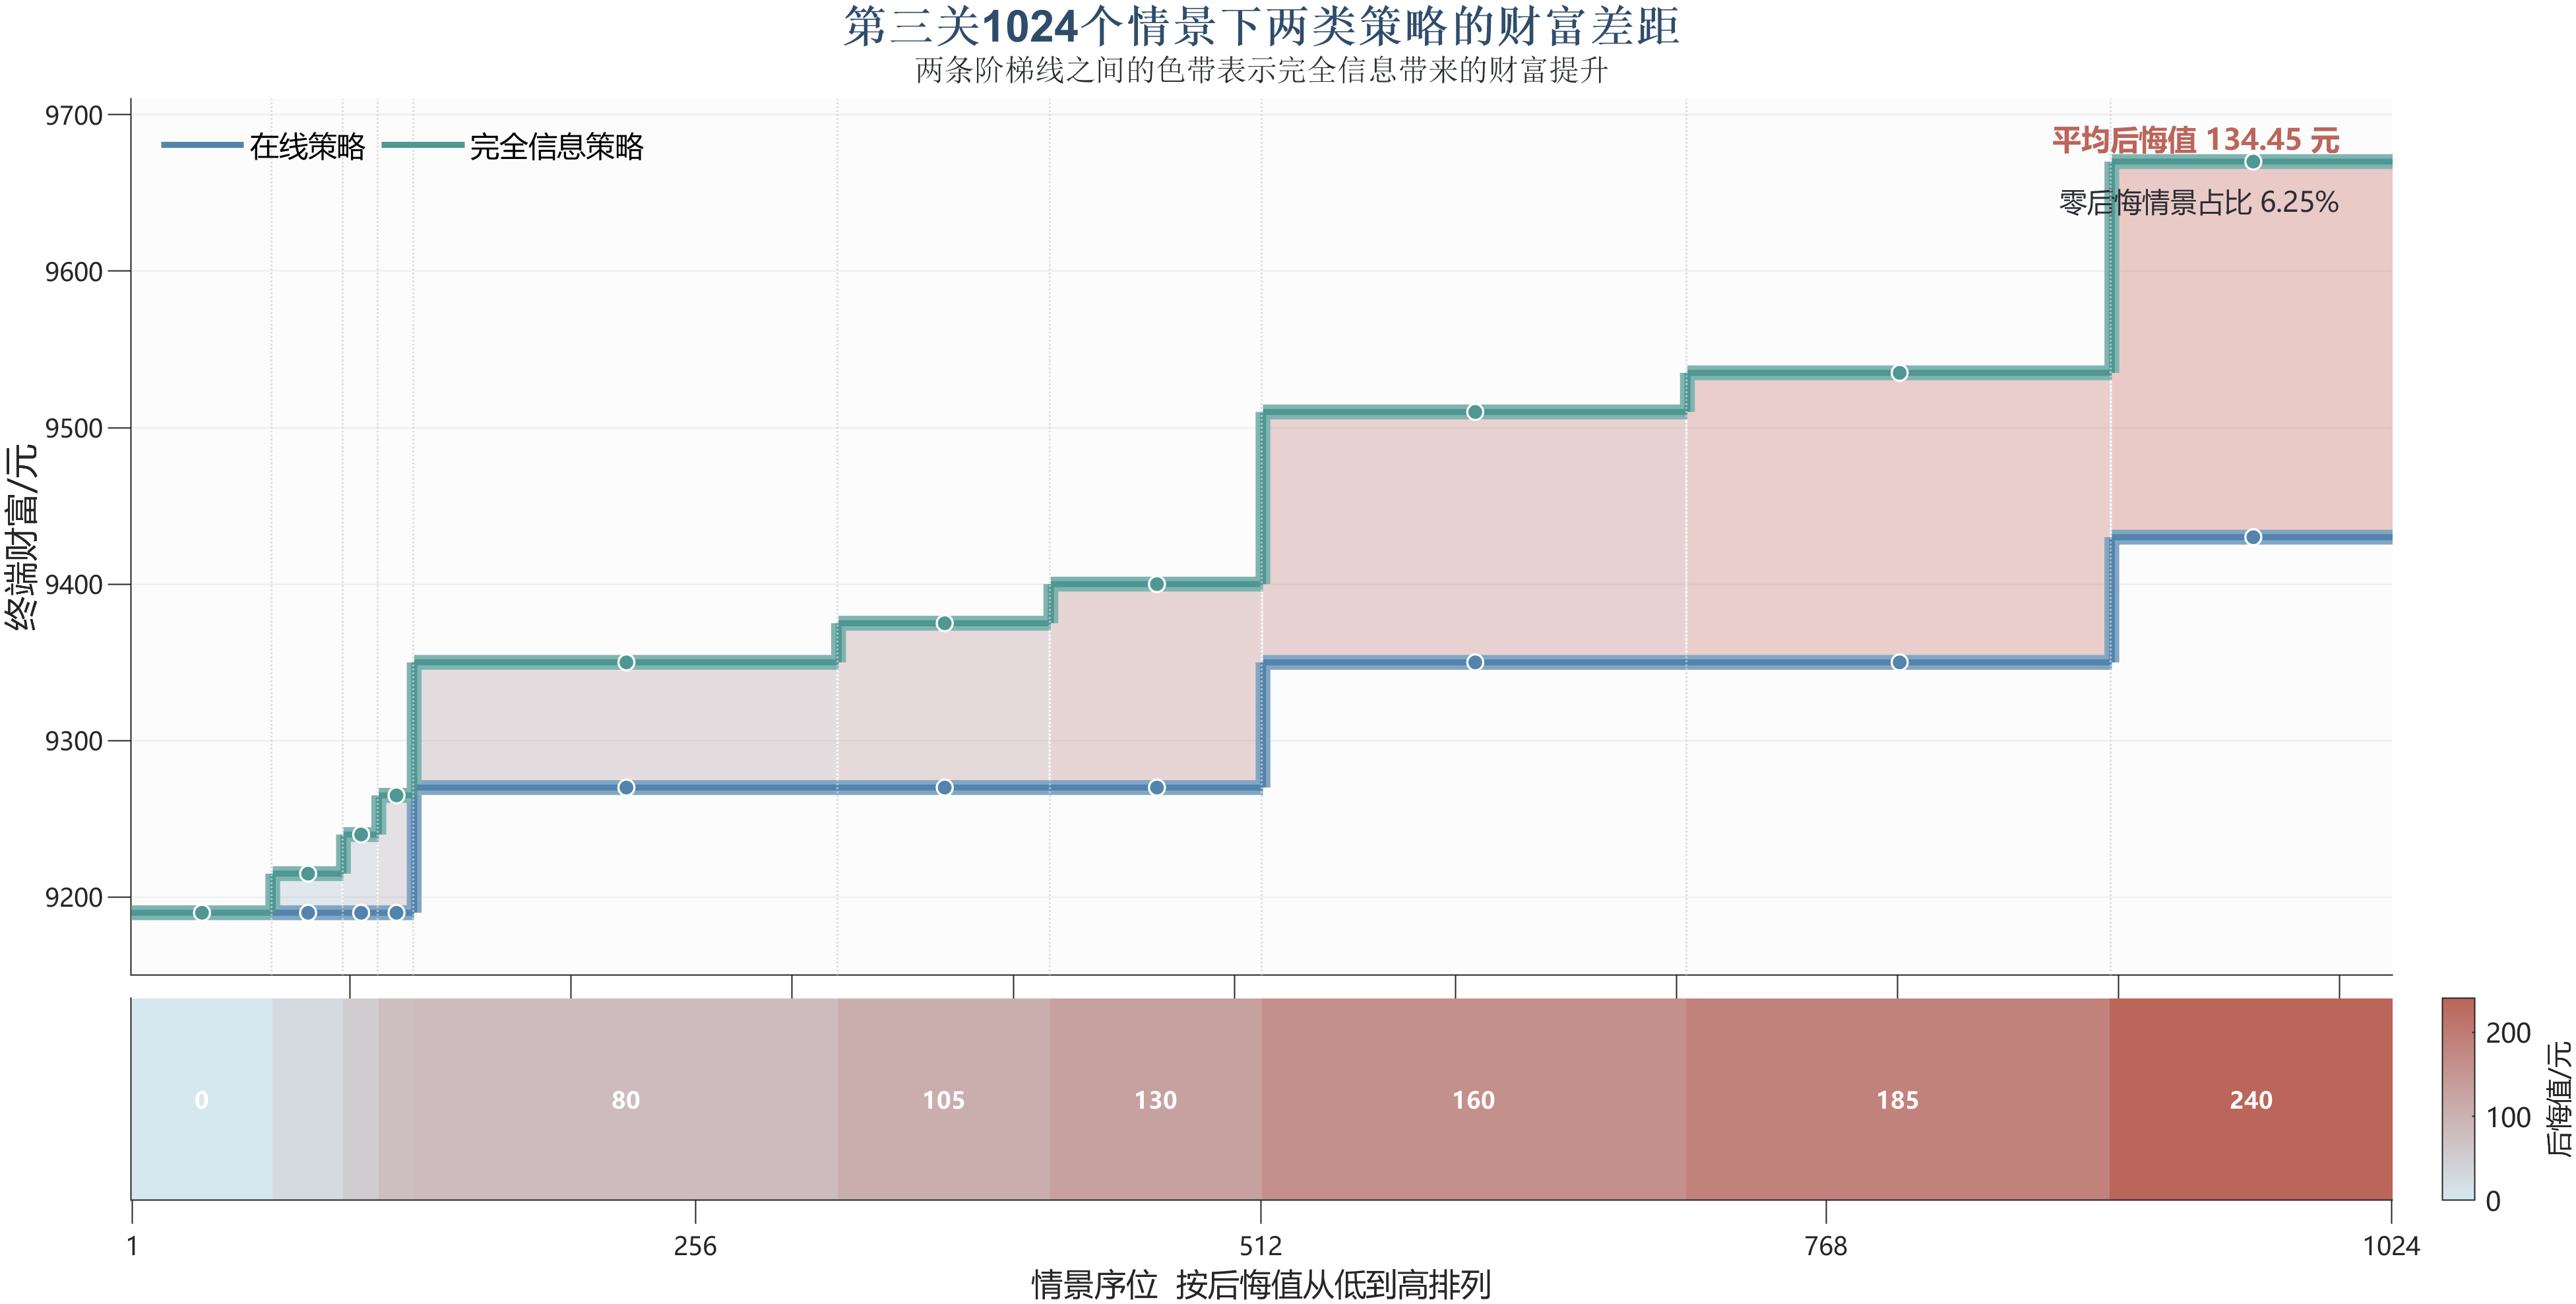
\includegraphics[width=\linewidth]{fig_q2_scenario_heatmap.png}
        \caption{1024个情景下在线与完全信息策略的财富差距}
    \end{subfigure}\hfill
    \begin{subfigure}[t]{0.32\textwidth}
        \centering
        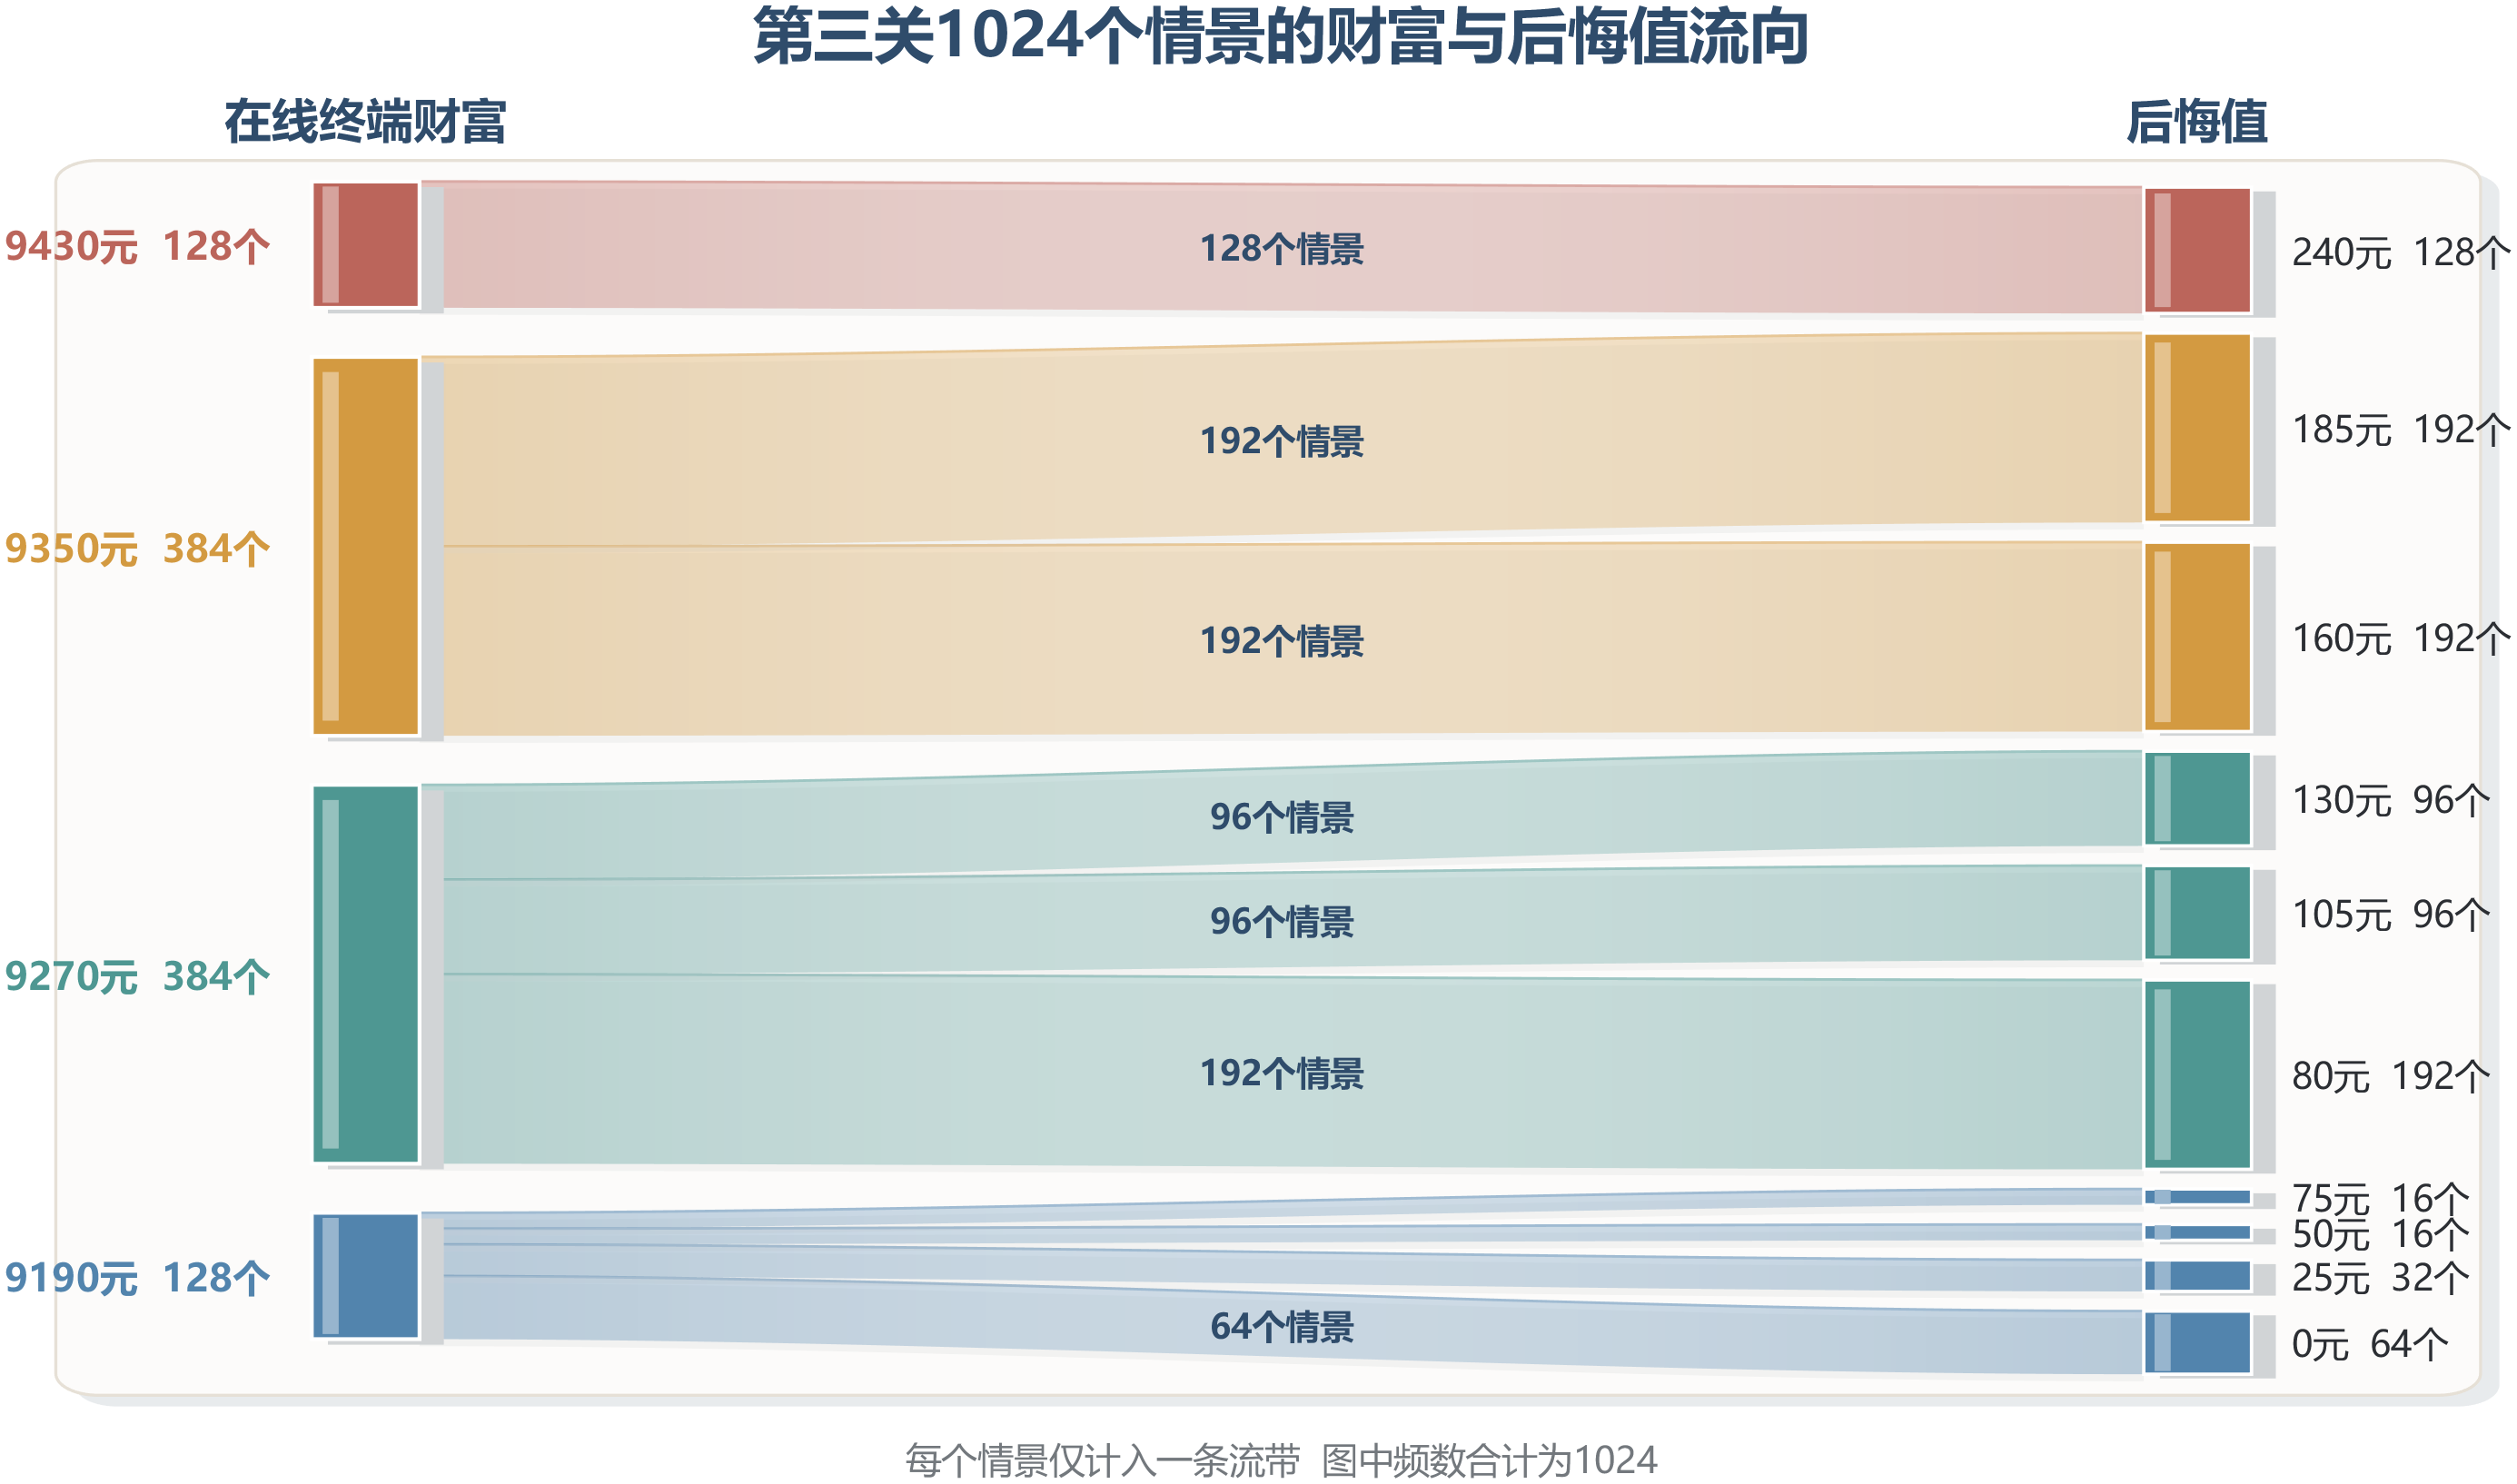
\includegraphics[width=\linewidth]{fig_q2_regret_distribution.png}
        \caption{1024个情景的财富与后悔值流向}
    \end{subfigure}
    \caption{第三关非前视鲁棒策略的可视化分析}
    \label{fig:q2_q3_analysis}
\end{figure}

图~\ref{fig:q2_q3_analysis}(a) 展示了第三关前三日的非前视决策树：第0日统一采购水、食各54箱后，前两日依据当天天气（晴朗/高温）逐日决定去向，第3日全部到达终点，8个叶节点各自包含128条完整情景。决策树下方矩阵对比了8个叶节点的在线财富、完全信息财富与后悔值均值，最坏叶节点（前三日连续高温）恰好耗尽54箱水食、对应财富9190元。图~\ref{fig:q2_q3_analysis}(b) 将1024条情景按后悔值升序排列，在线策略与完全信息策略两条财富阶梯之间的差距带整体收窄，平均后悔值仅134.45元，表明非前视约束带来的信息损失有限。图~\ref{fig:q2_q3_analysis}(c) 进一步以流带形式刻画财富层级到后悔值层级的流向：绝大多数情景集中在高财富、低后悔的流带，只有高温密集的情景落入最低财富档。

\textbf{第四关：}

第四关将"沙暴较少"的定性语义参数化为$\Gamma$，对$\Gamma=0,\dots,6$逐一求解，得到可行性与安全下界前沿。

\begin{table}[H]
    \centering
    \begin{tabular*}{\textwidth}{@{\extracolsep{\fill}}cccc}
        \toprule
        $\Gamma$ & 初购（水,食）/箱 & 保证财富下界/元 & 最迟保证到达日 \\
        \midrule
        0 & 144 & 7840 & 8 \\
        1 & 154 & 7690 & 9 \\
        2 & 164 & 7540 & 10 \\
        3 & 174 & 7390 & 11 \\
        4 & 184 & 7240 & 12 \\
        5 & 194 & 7090 & 13 \\
        \textbf{6} & \textbf{204} & \textbf{6940} & \textbf{14} \\
        \bottomrule
    \end{tabular*}
    \caption{第四关$\Gamma$预算鲁棒模型的安全下界前沿}
    \label{tab:q2_q4_frontier}
\end{table}

由表~\ref{tab:q2_q4_frontier}可知：$\Gamma=6$为推荐锚点；所有$\Gamma$共用同一8步最短路$1\to2\to3\to4\to5\to10\to15\to20\to25$。随$\Gamma$每增加1，初始采购同步增加10箱水、10箱食物，保证财富下界下降150元，最迟保证到达日推迟1天。需注意，本表为预算鲁棒模型的可证明安全下界，未包含村庄补给与矿山收益的全局最优鲁棒前沿。

\begin{figure}[H]
    \centering
    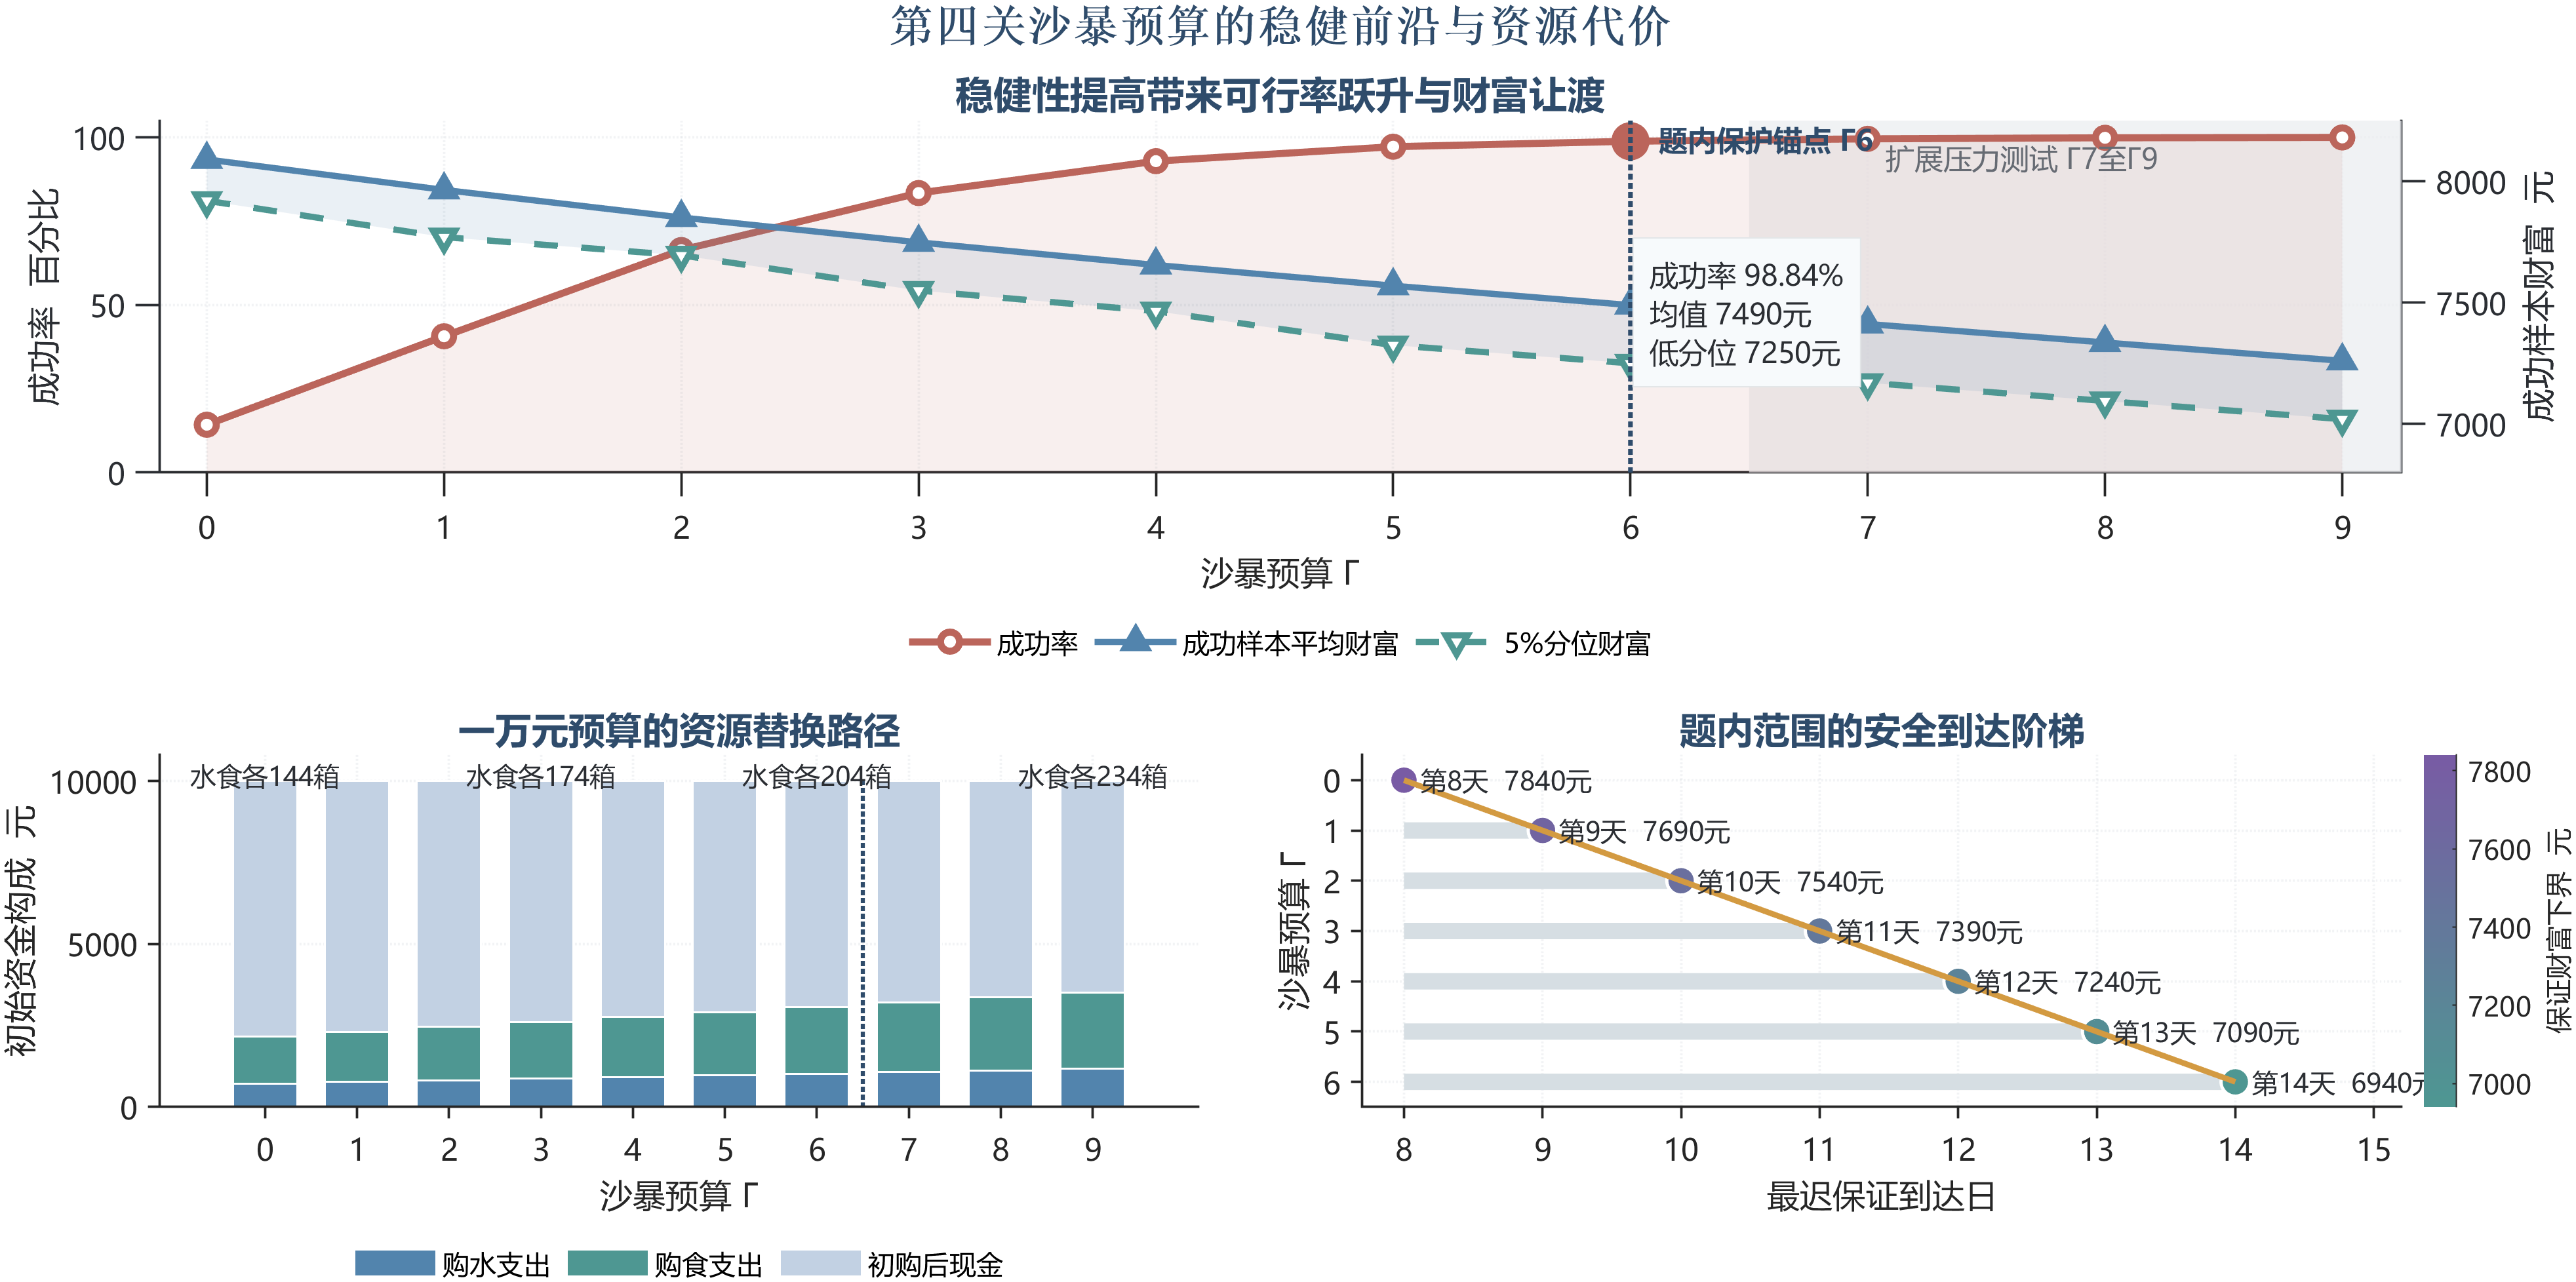
\includegraphics[width=0.98\textwidth]{fig_q2_q4_robust_frontier.png}
    \caption{第四关沙暴预算的稳健前沿与资源代价}
    \label{fig:q2_robust_frontier}
\end{figure}

\begin{figure}[H]
    \centering
    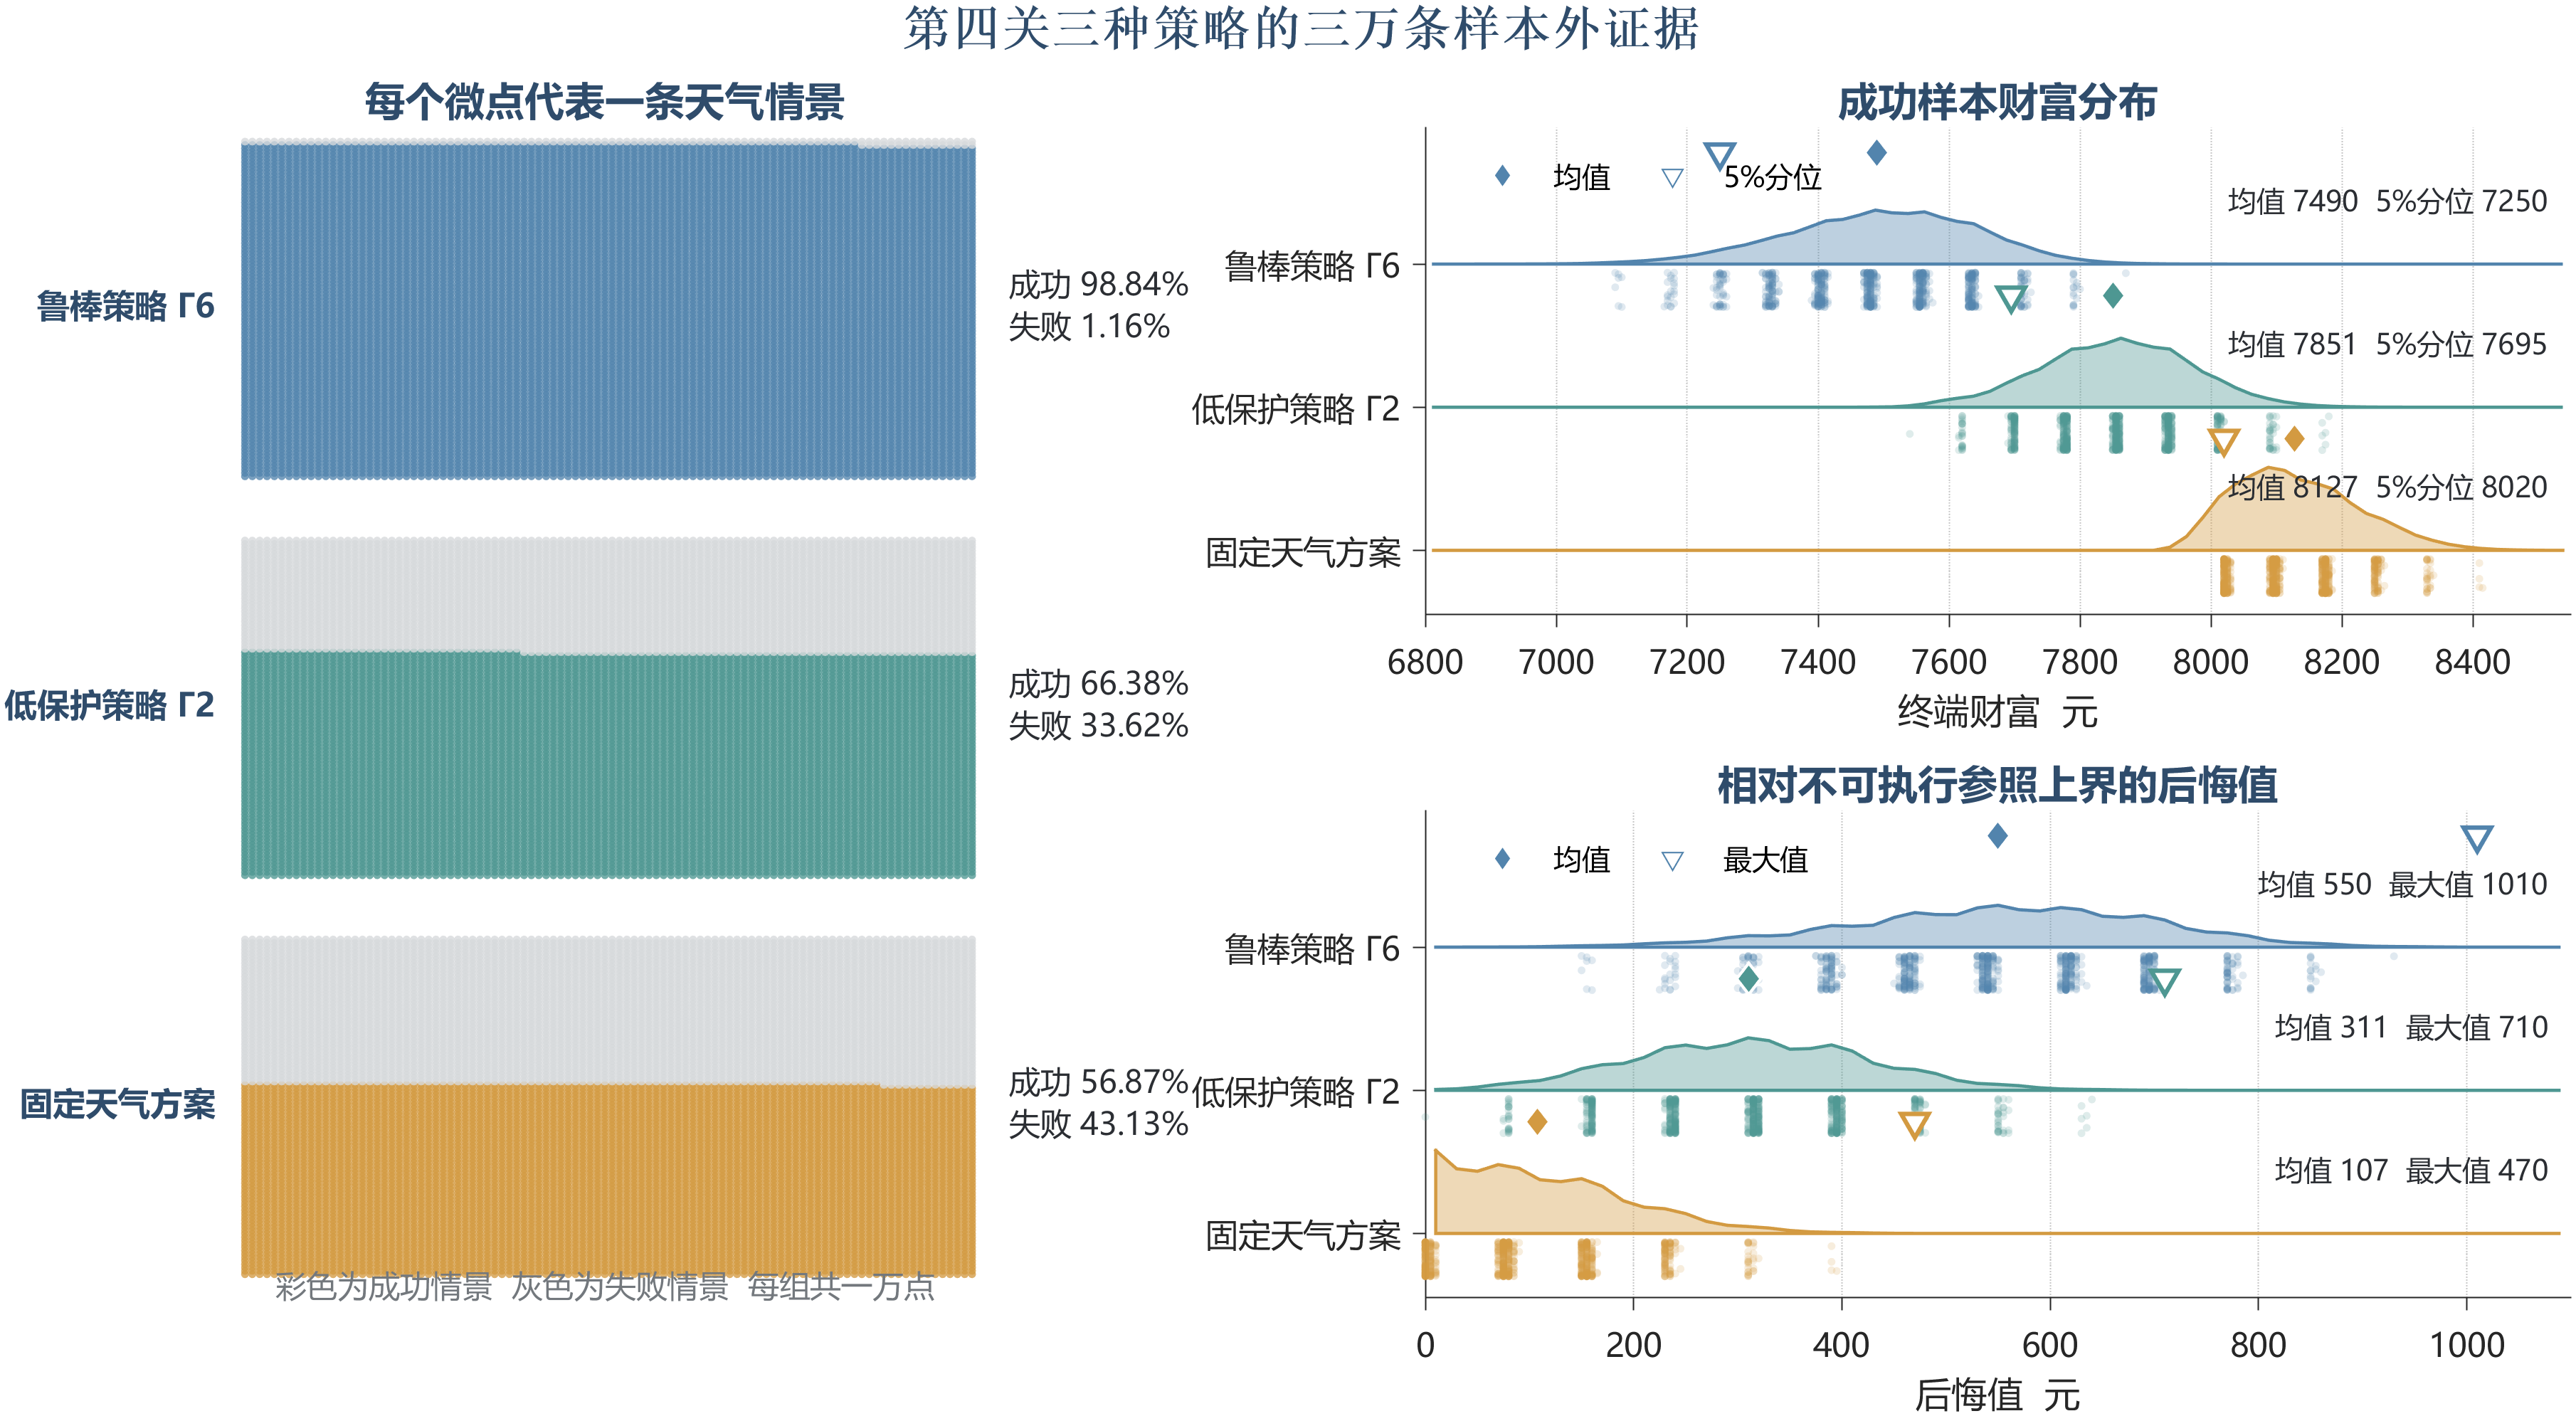
\includegraphics[width=0.98\textwidth]{fig_q2_q4_strategy_evidence.png}
    \caption{第四关三种策略的三万条样本外证据}
    \label{fig:q2_strategy_evidence}
\end{figure}

\begin{figure}[H]
    \centering
    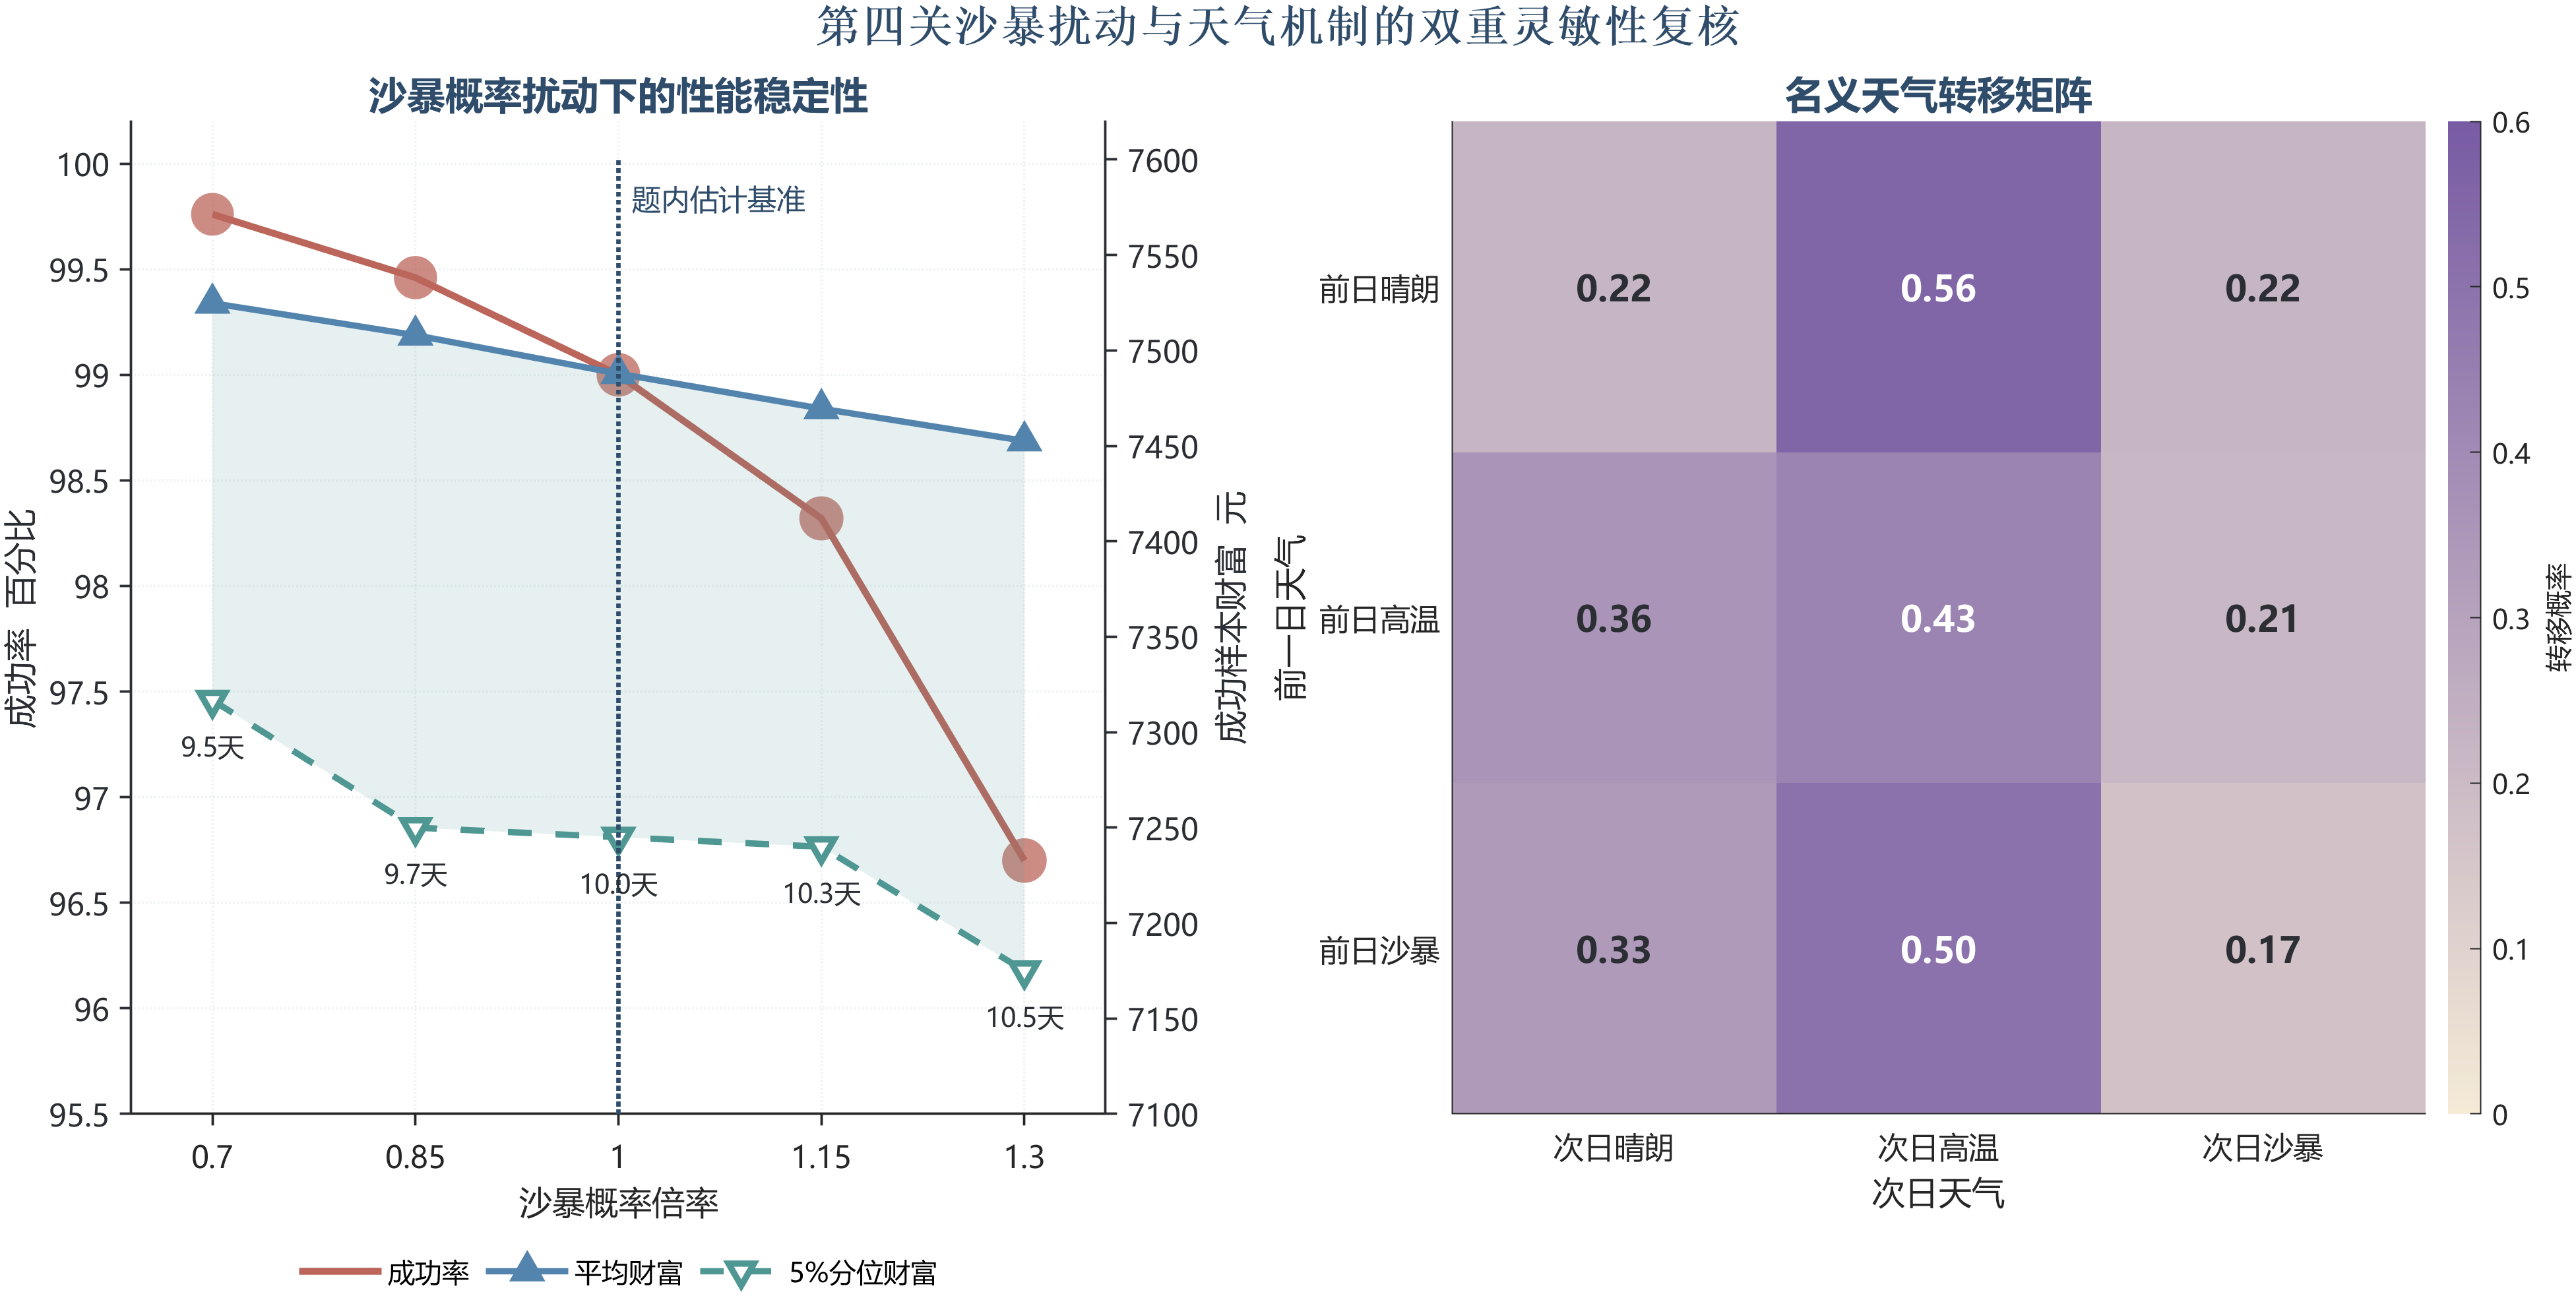
\includegraphics[width=0.98\textwidth]{fig_q2_q4_robustness_validation.png}
    \caption{第四关沙暴扰动与天气机制的双重灵敏性复核}
    \label{fig:q2_robustness_validation}
\end{figure}

图~\ref{fig:q2_robust_frontier} 呈现了$\Gamma=0,\dots,9$下的稳健前沿：随沙暴预算增大，成功率由14.27\%单调升至99.98\%，但成功样本平均财富由8090元降至7260元，形成清晰的"安全—收益"权衡；$\Gamma=6$作为题内数据锚定（历史含6个沙暴日）取得成功率98.84\%、平均财富7490元、5\%分位7250元的折中。图~\ref{fig:q2_strategy_evidence} 以一万点微点矩阵对比三种策略：鲁棒策略$\Gamma=6$几乎全为成功（98.84\%），而第一问固定天气方案与低保护方案$\Gamma=2$分别出现43.13\%与33.62\%的失败区；固定方案虽在成功样本上平均财富更高（8127元），但该条件均值排除了大量失败样本，不能单独作为策略优劣依据。图~\ref{fig:q2_robustness_validation} 对Markov矩阵沙暴列权重做0.7--1.3倍扰动后重抽样，沙暴概率提高30\%时成功率仍达96.70\%、平均到达日仅延至10.51天，主要结论未反转，说明策略不依赖Markov单点估计；右侧热力矩阵直观展示了晴朗/高温/沙暴之间的一阶转移结构。

\subsubsection{最优性验证}

对第二问采取与第一问一致的多层验证机制。首先由独立checker对全部输出轨迹逐日复算资源守恒、负重约束、购买规则、沙暴禁行与矿山动作合法性，两关均未发现违规。其次进行非前视断言检验：对任意两条可见历史相同的路径，断言其动作相同，程序返回非前视性成立。再次，第三关穷举全部1024条允许天气序列执行同一在线策略，失败数为0，并逐序列计算完全信息Oracle后悔值；第四关在$\Gamma$压力情景下进行最坏情形检验。逻辑上所有模型共享同一转移函数，保证了跨模型规则一致。

\subsubsection{灵敏性分析}

针对第二问不确定性的来源设计三层灵敏性分析。其一是$\Gamma$敏感性：表~\ref{tab:q2_q4_frontier} 已显示初购量、保证财富与最迟到达日随$\Gamma$单调变化，若在某一$\Gamma$区间内首日采购与关键动作保持不变，则该策略对"沙暴较少"的具体解释不敏感，可优先推荐。其二是转移矩阵扰动：对$\hat{P}$行概率做bootstrap扰动，检验名义期望的稳定性。其三是Monte Carlo评价：按$\hat{P}_4$生成大量天气序列，对在线策略统计成功率、平均财富、标准差、5\%分位与CVaR，衡量鲁棒策略为降低风险付出的平均收益代价。

\subsubsection{第二问结论}

综合上述建模与求解，第二问得到以下结论：

\textbf{第一，}在天气信息逐日揭示、未来天气不可见的条件下，自适应鲁棒动态规划将决策对象由固定路线推广为满足非前视约束的反馈策略，不依赖任何人为天气概率，所得策略对题面信息结构具有可解释性。

\textbf{第二，}第三关在1024种无沙暴天气序列上全部成功到达，最坏终端财富9190元，与完全信息Oracle相比后悔值中位数仅145元，说明"仅知当天"信息结构下的策略损失有限，具有强近优性。

\textbf{第三，}第四关将"沙暴较少"的模糊语义参数化为$\Gamma$预算不确定集，得到的稳健前沿单调且可解释，并给出可证明的安全下界；结合名义Markov模型的Monte Carlo评价，能够在"稳健安全"与"名义收益"之间给出客观取舍依据。
\section{参考文献与引用}

参考文献对于一篇正式的论文来说是必不可少的，在建模中重要的参考文献当然应该列出。\LaTeX{}在这方面的功能也是十分强大的，下面进介绍一个比较简单的参考文献制作方法。有兴趣的可以学习 \verb|bibtex| 或 \verb|biblatex| 的使用。

\LaTeX{}的入门书籍可以看《\LaTeX{}入门》\cite{liuhaiyang2013latex}。这是一个简单的引用，用 \verb|\cite{bibkey}| 来完成。要引用成功，当然要维护好 bibitem 了。下面是个简单的例子。

%参考文献
\begin{thebibliography}{9}%宽度9
    \bibitem[1]{liuhaiyang2013latex}
    刘海洋.
    \newblock \LaTeX {}入门\allowbreak[J].
    \newblock 电子工业出版社, 北京, 2013.
    \bibitem[2]{mathematical-modeling}
    全国大学生数学建模竞赛论文格式规范 (2020 年 8 月 25 日修改).
\end{thebibliography}

\newpage
%附录
\begin{appendices}
\section{第一问两关逐日最优决策}

两关逐日最优决策分别见表~\ref{tab:q1_daily1} 与表~\ref{tab:q1_daily2}，其中“购买(水,食)”仅在村庄补给日非零，“--”表示当日无采购。

{
\begin{longtable}{cccccccc} 
     \caption{第一关逐日最优决策表}
      \label{tab:q1_daily1} \\
    \toprule
    日期 & 天气 & 行动 & 所在区域 & 购买(水,食) & 剩余资金/元 & 剩余水量/箱 & 剩余食物量/箱 \\
    \midrule
    \endfirsthead
    \multicolumn{8}{c}{表~\ref{tab:q1_daily1}（续）} \\
    \toprule
    日期 & 天气 & 行动 & 所在区域 & 购买(水,食) & 剩余资金/元 & 剩余水量/箱 & 剩余食物量/箱 \\
    \midrule
    \endhead
    \midrule
    \multicolumn{8}{r}{续下页} \\
    \endfoot
    \bottomrule
    \endlastfoot
    0 & — & 起点采购 & 1 & 178,333 & 5780 & 178 & 333 \\
    1 & 高温 & 行走 & 25 & -- & 5780 & 162 & 321 \\
    2 & 高温 & 行走 & 24 & -- & 5780 & 146 & 309 \\
    3 & 晴朗 & 行走 & 23 & -- & 5780 & 136 & 295 \\
    4 & 沙暴 & 停留 & 23 & -- & 5780 & 126 & 285 \\
    5 & 晴朗 & 行走 & 21 & -- & 5780 & 116 & 271 \\
    6 & 高温 & 行走 & 9 & -- & 5780 & 100 & 259 \\
    7 & 沙暴 & 停留 & 9 & -- & 5780 & 90 & 249 \\
    8 & 晴朗 & 行走 & 15 & 163,0 & 4150 & 243 & 235 \\
    9 & 高温 & 行走 & 13 & -- & 4150 & 227 & 223 \\
    10 & 高温 & 行走 & 12 & -- & 4150 & 211 & 211 \\
    11 & 沙暴 & 停留 & 12 & -- & 4150 & 201 & 201 \\
    12 & 高温 & 挖矿 & 12 & -- & 5150 & 177 & 183 \\
    13 & 晴朗 & 挖矿 & 12 & -- & 6150 & 162 & 162 \\
    14 & 高温 & 挖矿 & 12 & -- & 7150 & 138 & 144 \\
    15 & 高温 & 挖矿 & 12 & -- & 8150 & 114 & 126 \\
    16 & 高温 & 挖矿 & 12 & -- & 9150 & 90 & 108 \\
    17 & 沙暴 & 停留 & 12 & -- & 9150 & 80 & 98 \\
    18 & 沙暴 & 挖矿 & 12 & -- & 10150 & 50 & 68 \\
    19 & 高温 & 挖矿 & 12 & -- & 11150 & 26 & 50 \\
    20 & 高温 & 行走 & 13 & -- & 11150 & 10 & 38 \\
    21 & 晴朗 & 行走 & 15 & 36,16 & 10470 & 36 & 40 \\
    22 & 晴朗 & 行走 & 9 & -- & 10470 & 26 & 26 \\
    23 & 高温 & 行走 & 21 & -- & 10470 & 10 & 14 \\
    24 & 晴朗 & 行走 & 27 & -- & 10470 & 0 & 0 \\
   
\end{longtable}
}

{
\begin{longtable}{cccccccc}
    \caption{第二关逐日最优决策表}
      \label{tab:q1_daily2} \\
    \toprule
    日期 & 天气 & 行动 & 所在区域 & 购买(水,食) & 剩余资金/元 & 剩余水量/箱 & 剩余食物量/箱 \\
    \midrule
    \endfirsthead
    \multicolumn{8}{c}{表~\ref{tab:q1_daily2}（续）} \\
    \toprule
    日期 & 天气 & 行动 & 所在区域 & 购买(水,食) & 剩余资金/元 & 剩余水量/箱 & 剩余食物量/箱 \\
    \midrule
    \endhead
    \midrule
    \multicolumn{8}{r}{续下页} \\
    \endfoot
    \bottomrule
    \endlastfoot
    0 & — & 起点采购 & 1 & 130,405 & 5300 & 130 & 405 \\
    1 & 高温 & 行走 & 9 & -- & 5300 & 114 & 393 \\
    2 & 高温 & 行走 & 18 & -- & 5300 & 98 & 381 \\
    3 & 晴朗 & 行走 & 26 & -- & 5300 & 88 & 367 \\
    4 & 沙暴 & 停留 & 26 & -- & 5300 & 78 & 357 \\
    5 & 晴朗 & 行走 & 27 & -- & 5300 & 68 & 343 \\
    6 & 高温 & 行走 & 36 & -- & 5300 & 52 & 331 \\
    7 & 沙暴 & 停留 & 36 & -- & 5300 & 42 & 321 \\
    8 & 晴朗 & 行走 & 37 & -- & 5300 & 32 & 307 \\
    9 & 高温 & 行走 & 38 & -- & 5300 & 16 & 295 \\
    10 & 高温 & 行走 & 39 & 10,0 & 5200 & 10 & 283 \\
    11 & 沙暴 & 停留 & 39 & 218,0 & 3020 & 218 & 273 \\
    12 & 高温 & 行走 & 30 & -- & 3020 & 202 & 261 \\
    13 & 晴朗 & 挖矿 & 30 & -- & 4020 & 187 & 240 \\
    14 & 高温 & 挖矿 & 30 & -- & 5020 & 163 & 222 \\
    15 & 高温 & 挖矿 & 30 & -- & 6020 & 139 & 204 \\
    16 & 高温 & 挖矿 & 30 & -- & 7020 & 115 & 186 \\
    17 & 沙暴 & 挖矿 & 30 & -- & 8020 & 85 & 156 \\
    18 & 沙暴 & 挖矿 & 30 & -- & 9020 & 55 & 126 \\
    19 & 高温 & 行走 & 39 & 157,86 & 5730 & 196 & 200 \\
    20 & 高温 & 行走 & 46 & -- & 5730 & 180 & 188 \\
    21 & 晴朗 & 行走 & 55 & -- & 5730 & 170 & 174 \\
    22 & 晴朗 & 挖矿 & 55 & -- & 6730 & 155 & 153 \\
    23 & 高温 & 挖矿 & 55 & -- & 7730 & 131 & 135 \\
    24 & 晴朗 & 挖矿 & 55 & -- & 8730 & 116 & 114 \\
    25 & 沙暴 & 挖矿 & 55 & -- & 9730 & 86 & 84 \\
    26 & 高温 & 挖矿 & 55 & -- & 10730 & 62 & 66 \\
    27 & 晴朗 & 挖矿 & 55 & -- & 11730 & 47 & 45 \\
    28 & 晴朗 & 挖矿 & 55 & -- & 12730 & 32 & 24 \\
    29 & 高温 & 行走 & 56 & -- & 12730 & 16 & 12 \\
    30 & 高温 & 行走 & 64 & -- & 12730 & 0 & 0 \\
     
\end{longtable}
}




\end{appendices}
\end{document} 